%%%%%%%%%%%%%%%%%%%%%%%%%%%%%%%%%%%%%%%%%%%%%%%%%%%%%%%%%%%%%%%%%%%%%%%%%%%%%%%%%%%%%%%%%%%%%%%%%%%%%%%%%%%%%%%%%%%%%%%%%%%%%%%%%%%%%%%%%%%%%%%%%%%%%%%%%%%
% This is just an example/guide for you to refer to when submitting manuscripts
% to Frontiers, it is not mandatory to use Frontiers .cls files nor
% frontiers.tex  % This will only generate the Manuscript, the final article
% will be typeset by Frontiers after acceptance.
%                                              %
%                                                                                                                                                         %
% When submitting your files, remember to upload this *tex file, the pdf
% generated with it, the *bib file (if bibliography is not within the *tex) and
% all the figures.
%%%%%%%%%%%%%%%%%%%%%%%%%%%%%%%%%%%%%%%%%%%%%%%%%%%%%%%%%%%%%%%%%%%%%%%%%%%%%%%%%%%%%%%%%%%%%%%%%%%%%%%%%%%%%%%%%%%%%%%%%%%%%%%%%%%%%%%%%%%%%%%%%%%%%%%%%%%

% Version 3.3 Generated 2016/11/10 %%% You will need to have the following
% packages installed: datetime, fmtcount, etoolbox, fcprefix, which are
% normally inlcuded in WinEdt. %%% In http://www.ctan.org/ you can find the
% packages and how to install them, if necessary. %%% NB logo1.jpg is required
% in the path in order to correctly compile front page header %%%

\documentclass[utf8]{frontiersSCNS} % for Science, Engineering and Humanities and Social Sciences articles
%\documentclass[utf8]{frontiersHLTH} % for Health articles
%\documentclass[utf8]{frontiersFPHY} % for Physics and Applied Mathematics and Statistics articles

%\setcitestyle{square} % for Physics and Applied Mathematics and Statistics articles
\usepackage{url,hyperref,lineno,microtype,subcaption}
\usepackage[onehalfspacing]{setspace}
%\usepackage{todonotes}
%\newcommand{\todoil}[1]{\todo[inline]{#1}}

\usepackage[utf8]{inputenc}
\usepackage{hyperref}
\usepackage{microtype}
\usepackage{letltxmacro}
\usepackage[cmintegrals,cmbraces]{newtxmath}

\usepackage{booktabs}
\usepackage{mathtools}
\usepackage{amssymb}
\usepackage{tikz}
%\usepackage{enumitem}
\usepackage{multirow}
\usepackage{rotating}
\usepackage{placeins}
\usepackage[textsize=miniscule, linecolor=magenta, bordercolor=magenta,
            backgroundcolor=magenta, textwidth=1.1cm]{todonotes}

%\linenumbers

\makeatletter

\ifcase \@ptsize \relax% 10pt
  \newcommand{\miniscule}{\@setfontsize\miniscule{4}{5}}% \tiny: 5/6
\or% 11pt
  \newcommand{\miniscule}{\@setfontsize\miniscule{5}{6}}% \tiny: 6/7
\or% 12pt
  \newcommand{\miniscule}{\@setfontsize\miniscule{5}{6}}% \tiny: 6/7
\fi

    \renewcommand{\@todonotes@drawMarginNoteWithLine}{%
    \begin{tikzpicture}[remember picture, overlay, baseline=-0.75ex]%
        \node [coordinate] (inText) {};%
    \end{tikzpicture}%
    \marginpar[{% Draw note in left margin
        \@todonotes@drawMarginNote{r}%
        \@todonotes@drawLineToLeftMargin%
    }]{% Draw note in right margin
        \@todonotes@drawMarginNote{l}%
        \@todonotes@drawLineToRightMargin%
    }%
    }
    \renewcommand{\@todonotes@drawMarginNote}[1]{
        \makebox[\marginparwidth][#1]{\begin{tikzpicture}[remember picture,baseline=(X.base)]%
            \node(X){\vphantom{X}};%
            \draw node[notestyle,font=\@todonotes@sizecommand,anchor=north] (inNote) at (X.north)%
                {\@todonotes@text};%
            \if@todonotes@authorgiven%
                \draw node[notestyle,font=\@todonotes@sizecommand,anchor=north] (inNote) at (X.north)%
                    {\@todonotes@sizecommand\@todonotes@author};%
                \node(Y)[below=of X]{};%
                \draw node[notestyle,font=\@todonotes@sizecommand,anchor=north] (inNote) at (X.south)%
                    {\@todonotes@text};%
            \else%
                \draw node[notestyle,font=\@todonotes@sizecommand,anchor=north] (inNote) at (X.north)%
                    {\@todonotes@text};%
            \fi%
        \end{tikzpicture}%
    }}
\makeatother
\LetLtxMacro{\oldtodo}{\todo}
\renewcommand{\todo}[1]{{\miniscule \color{magenta}\oldtodo[fancyline]{ \color{white}\textsf{#1} }}}
\newcommand{\inlinetodo}[1]{{\color{magenta}\oldtodo[inline]{\color{white}\textsf{\small#1}}}}

\def\keyFont{\fontsize{8}{11}\helveticabold }
\def\firstAuthorLast{Lampa {et~al.}} %use et al only if is more than 1 author
\def\Authors{Samuel Lampa\,$^{1,*}$, Jonathan Alvarsson\,$^{1}$, Staffan Arvidsson Mc Shane\,$^{1}$, Arvid Berg\,$^{1}$, Ernst Ahlberg\,$^{2}$  and Ola Spjuth\,$^{1}$}
% Affiliations should be keyed to the author's name with superscript numbers
% and be listed as follows: Laboratory, Institute, Department, Organization,
% City, State abbreviation (USA, Canada, Australia), and Country (without
% detailed address information such as city zip codes or street names).  If one
% of the authors has a change of address, list the new address below the
% correspondence details using a superscript symbol and use the same symbol to
% indicate the author in the author list.
\def\Address{$^{1}$Pharmaceutical Bioinformatics group, Department of Pharmaceutical Biosciences, Uppsala University, Uppsala, Sweden\\
$^{2}$Predictive Compound ADME \& Safety, Drug Safety \& Metabolism, AstraZeneca IMED Biotech Unit, M\"olndal, Sweden}
% The Corresponding Author should be marked with an asterisk Provide the exact
% contact address (this time including street name and city zip code) and email
% of the corresponding author
\def\corrAuthor{Corresponding Author}

\def\corrEmail{samuel.lampa@farmbio.uu.se}


\begin{document}

\onecolumn
\firstpage{1}

\title[Predicting off-target binding profiles with confidence using Conformal
Prediction]{Predicting off-target binding profiles with confidence using Conformal
Prediction}

\author[\firstAuthorLast ]{\Authors} %This field will be automatically populated
\address{} %This field will be automatically populated
\correspondance{} %This field will be automatically populated

\extraAuth{}% If there are more than 1 corresponding author, comment this line and uncomment the next one.
%\extraAuth{corresponding Author2 \\ Laboratory X2, Institute X2, Department
%X2, Organization X2, Street X2, City X2 , State XX2 (only USA, Canada and
%Australia), Zip Code2, X2 Country X2, email2@uni2.edu}


\maketitle


\begin{abstract}

%%% Leave the Abstract empty if your article does not require one, please see the Summary Table for full details.
%\section{}
%For full guidelines regarding your manuscript please refer to
%    \href{http://www.frontiersin.org/about/AuthorGuidelines}{Author
%    Guidelines}.
%
%As a primary goal, the abstract should render the general significance and
%    conceptual advance of the work clearly accessible to a broad readership.
%    References should not be cited in the abstract. Leave the Abstract empty if
%    your article does not require one, please see
%    \href{http://www.frontiersin.org/about/AuthorGuidelines#SummaryTable}{Summary
%    Table} for details according to article type.

%\todoil{Can you really have refs in abstract?}
%\todoil{--- No not really, the abstract should probably be completely rewritten. // jonalv}
%\todoil{--- No refs and no abbreviations. /Ola}
%Off-target pharmacology and polypharmacology has big implications on drug
%efficacy and safety, and prediction of target binding profiles for ligands is
%an important task that can aid early drug discovery \cite{Bowes2012}.
%However, available methods for ligand-based target profiling do not offer
%valid measures of confidence in predictions or well-calibrated probabilities.
%We present an approach for ligand-based target profiling using probabilistic
%predictions, delivering target profiles with valid predictions of the
%probability for the query compound to interact with each target. The
%probabilities are calculated using the Conformal Prediction methodology
%\cite{Vovk2005}, with support vector machines for modeling and chemical
%structures described by the signature molecular descriptor \cite{Faulon2003}.
%We study profiles for different sets of targets, including a subset of the
%minimal panel of 44 targets for broad early hazard assessment suggested by
%\cite{Bowes2012}, but also the applicability of larger as well as focused
%target sets. The resulting method is available as an online Web service via
%an API, and we also make the complete workflow for reproducing the study
%together with all models publicly available.

Ligand-based models can be used in drug discovery to obtain an early indication
of potential off-target interactions that could be linked to adverse
effects. Another application is to combine such models into a panel,
allowing for comparing and searching for compounds with similar profile. Most
contemporary methods and implementations however lack valid measures of
confidence in predictions, presenting only point predictions. We here
describe the use of conformal prediction for predicting off-target
interactions with models trained on data from 31 targets in the ExCAPE
database, selected for their utility in broad early hazard assessment.
Chemicals were represented by the signature molecular descriptor and
support vector machines were used as the underlying machine learning method. With
conformal prediction, results from predictions are in the form of confidence
p-values for each class.  The full pre-processing and model training
process is openly available as a scientific workflow on GitHub, rendering it
fully reproducible.  We illustrate the usefulness of the methodology on a set
of compounds extracted from DrugBank.  The resulting models are published
online and are available via a graphical web interface and an OpenAPI interface
for programmatic access.\todo{Push more on workflow as a method?}

\tiny
 \keyFont{ \section{Keywords:} drug discovery, predictive modelling, conformal prediction, machine learning, off-target, adverse effects} %All article types: you may provide up to 8 keywords; at least 5 are mandatory.
\end{abstract}

\section*{Introduction}

%Introduce off target binding as a problem, and the value of predictions
Drug-target interactions are central to the drug discovery
process~\cite{Yildirim:2007vh}. It is common that drugs interact with multiple
targets~\cite{hopkins2008network}, and off-target pharmacology and
polypharmacology has important implications on drug efficacy and
safety~\cite{Peters:2013yg,Ravikumar:2018qd}. Organizations involved in drug
discovery, such as pharmaceutical companies and academic institutions, use many
types of experimental techniques and assays to determine target interactions,
including in vitro pharmacological profiling~\cite{Bowes2012}. However an
attractive complementary method is to use computational (in silico) profiling
of binding profiles for ligands~\cite{Cereto-Massague:2015px}, which also opens the possibility
to predict virtual compounds. A common approach to the target prediction
problem is to use a panel of structure-activity relationship (QSAR)
models~\cite{HanschQSAR}, where chemicals in a knowledge base with known
interaction values (numerical or categorial) are described numerically by
descriptors and a statistical learning model is trained to predict numerical
values (regression) or categorial values (classification). The recent increase
in the number of available data points in interaction databases such as ChEMBL~\cite{Gaulton:2017tm} and
PubChem~\cite{Wang:2017cy} makes it possible to using ligand-based models to predict not only targets but also panels of targets.

Several methods and tools are available for target prediction and for
constructing and using target profiles.
%
Bender \textit{et al}. use a Bayesian approach to train models for 70 selected targets
and use these for target profiling to classify adverse drug
reactions~\cite{Bender:2007ib}.
%
Yao \textit{et al}. describes TargetNet~\cite{Yao:2016ij}, a web service for
multi-target QSAR models; an online service that uses Na\"ive Bayes.
%
Yu \textit{et al}. use Random Forest (RF) and Support Vector Machines (SVM) to predict
drug-target interactions from heterogeneous biological data~\cite{Yu:2012ol}.
%
TargetHunter~\cite{Wang:2013le} is another online tool that uses chemical
similarity to predict targets for ligands, and show how training models on
ChEMBL data can enable useful predictions on examples taken from PubChem
bioassays.
%
The polypharmacology browser~\cite{Awale:2017is} is a web-based target
prediction tool that queries ChEMBL bioactivity data using multiple
fingerprints.


We note two important shortcomings among previous works. Primarily, available
methods for ligand-based target profiling often do not offer valid measures of
confidence in predictions, leaving the user uncertain about the usefulness of
predictions. Secondly, the majority of the web tools lack an open and
standardized API, meaning it is not straightforward (and in most cases not
possible at all) to consume the services programmatically, such as with a
script or inclusion in a scientific workflow management system used in drug discovery like
KNIME~\cite{Mazanetz:2012gy}.

We here present an approach for ligand-based target profiling using a
confidence framework, delivering target profiles with confidence scores for the
predictions of whether a query compound interacts with each target. The
confidence scores were calculated using the Conformal Prediction
methodology~\cite{Vovk2005}.
%
The goal of this study was to create an automated and reproducible approach for
generating a predicted target profile by QSAR binding models, with the models
making up the profile published online as microservices and the profile
accessible from a web page. Although the models give a confidence measure we
also set out to evaluate them on test sets to see how well they performed on some
representable data. We exemplified the process by creating a profile on the
targets for broad early hazard assessment presented by Bowes \textit{et
al.}~\cite{Bowes2012}.

%%%%%%%%%%%%%%%%%%
%Methods
%%%%%%%%%%%%%%%%%%
\section*{Methods}

\subsection*{Training data}

A scientific workflow was constructed to automate the entire data
preprocessing.  The first step comprised extracting data on binding association
between ligands and targets from the ExcapeDB dataset~\cite{Sun2017}, more
specifically the columns Gene name, Original entry ID (PubChem CID or CHEMBL
ID), SMILES and Activity flag. This was performed early in the workflow to make
subsequent data transformation steps less time-consuming, given the relatively large
size of the uncompressed ExcapeDB data file (18 GB).
%
From the extracted dataset, all rows for which there existed rows with a conflicting
activity value for the same target (gene symbol) and SMILES string, were completely removed.
% (See \footnote{\url{https://github.com/pharmbio/ptp-project/blob/c529cf/exp/20180426-wo-drugbank/wo\_drugbank\_wf.go\#L239-L246}}).

A subset of the panel of 44 binding targets as suggested in \cite{Bowes2012}
was selected for inclusion in the study. The selection was based on the
criteria that targets should have at least 100 active and at least 100
non-active compounds.  In addition some targets were excluded for which data
was not found in ExcapeDB. This is described in detail below.
%
Some of the gene symbols used in \cite{Bowes2012} were not found in their exact
form in the ExcapeDB dataset. To resolve this, PubMed was consulted to find
synonymous gene symbols with the following replacements done:
%
\textit{KCNE1} was replaced with \textit{MINK1} which is present in ExcapeDB.
\textit{CHRNA1} (coding for the $\alpha1$ subunit of the Acetylcholine
receptor) is excluded, as it is not present in the dataset (\textit{CHRNA4},
coding for the $\alpha4$ subunit of the Acetylcholine receptor, is present in
the dataset). We note that both \textit{MINK1} and \textit{CHRNA4} were removed
in the filtering step mentioned above, since the dataset did not contain more
than 100 active and 100 non-active compounds for \textit{MINK1} nor
\textit{CHRNA}.  However, since one aim of the study is to present and publish
an automated and reproducible data processing workflow, these targets could
potentially be included in subsequent runs on later versions of the database
with additional data available.

The resulting set (named Dataset1) consisted of 31 targets (marked as included in
Table~\ref{tbl:targets}).  For 21 of these targets, the dataset contained less
than 10\,000 non-active compounds, leading to imbalanced datasets (marked with
a \checkmark\ in the `Filled-up' column of Table~\ref{tbl:targets}).
%
For these 21 targets, we ``filled up'' their respective datasets with randomly
selected examples from the raw dataset which were not reported to be active for
this target, thus being `assumed non-active'. The number of new examples was chosen such that the total
number of non-actives and assumed non-actives added up to twice the number of
actives, for each target respectively. This dataset was named Dataset2.
The compounds for the remaining 10 targets, which were not filled-up, were
named Dataset3.
% (See
% \href{https://github.com/pharmbio/ptp-project/blob/c529cf307593c40e7f822a92b224036894c95de1/exp/20180426-wo-drugbank/wo_drugbank_wf.go#L308-L328}{here}
% for workflow code).
%
All the targets, with details about their respective number of active and
non-active compounds, and whether they are included or not, are summarized in
table~\ref{tbl:targets}.

\begin{table}[p]
\small
\centering
\caption{The panel of targets used in this study, identified by gene symbol.
    Actives and non-actives refer to the number of ligand interactions marked
    as active and non-active in ExcapeDB. Included indicates if the target was
    included in the study or excluded because it did not pass the filtering
    criteria.}
\label{tbl:targets}
\begin{tabular}{crrrrcl}
\toprule
&             &         & Non-actives       & Non-actives      &              &       \\
&             &         & (before fillup \& & (after fillup \& &              &       \\
& Gene symbol & Actives & deduplication)    & deduplication)   & Filled-up  & Remarks \\
\midrule
\multirow{31}{*}{\begin{turn}{90}\textsc{Included}\end{turn}}
&    ACHE    &       3\,160  &       1\,152      &   5\,824   & \checkmark      &       \\
&    ADORA2A &       5\,275  &       593         &   10\,092  & \checkmark      &       \\
&    ADRB1   &       1\,306  &       149         &   2\,544   & \checkmark      &       \\
&    ADRB2   &       1\,955  &       342\,282    &   341\,925 &       &       \\
&    AR      &       2\,593  &       4\,725      &   4\,866   & \checkmark      &       \\
&    AVPR1A  &       1\,055  &       321\,406    &   321\,098 &       &       \\
&    CCKAR   &       1\,249  &       132         &   2\,458   & \checkmark      &       \\
&    CHRM1   &       2\,776  &       417\,549    &   358\,330 &       &       \\
&    CHRM2   &       1\,817  &       152         &   3\,440   & \checkmark      &       \\
&    CHRM3   &       1\,676  &       144         &   3\,234   & \checkmark      &       \\
&    CNR1    &       5\,336  &       400         &   10\,220  & \checkmark      &       \\
&    CNR2    &       4\,583  &       402         &   8\,676   & \checkmark      &       \\
&    DRD1    &       1\,732  &       356\,201    &   355\,909 &       &       \\
&    DRD2    &       8\,323  &       343\,206    &   342\,958 &       &       \\
&    EDNRA   &       2\,129  &       124         &   4\,050   & \checkmark      &       \\
&    HTR1A   &       6\,555  &       64\,578     &   64\,468  &       &       \\
&    HTR2A   &       4\,160  &       359\,962    &   359\,663 &       &       \\
&    KCNH2   &       5\,330  &       350\,773    &   350\,452 &       &       \\
&    LCK     &       2\,662  &       283         &   5\,246   & \checkmark      &       \\
&    MAOA    &       1\,260  &       1\,083      &   2\,452   & \checkmark      &       \\
&    NR3C1   &       2\,525  &       4\,382      &   4\,804   & \checkmark      &       \\
&    OPRD1   &       5\,350  &       826         &   9\,580   & \checkmark      &       \\
&    OPRK1   &       3\,672  &       303\,335    &   303\,111 &       &       \\
&    OPRM1   &       5\,837  &       2\,872      &   11\,252  & \checkmark      &       \\
&    PDE3A   &       197     &       110         &   392      & \checkmark      &       \\
&    PTGS1   &       849     &       729         &   1\,634   & \checkmark      &       \\
&    PTGS2   &       2\,862  &       827         &   5\,162   & \checkmark      &       \\
&    SCN5A   &       316     &       119         &   624      & \checkmark      &       \\
&    SLC6A2  &       3\,879  &       218         &   7\,498   & \checkmark      &       \\
&    SLC6A3  &       5\,017  &       106\,819    &   106\,594 &       &       \\
&    SLC6A4  &       7\,228  &       382         &   13\,660  & \checkmark      &       \\
\midrule
\multirow{15}{*}{\begin{turn}{90}\textsc{Not Included}\end{turn}}
&    ADRA1A  &       1\,782  &       24          &            &       &       \\
&    ADRA2A  &       839     &       39          &            &       &       \\
&    CACNA1C &       166     &       20          &            &       &       \\
&    CHRNA1  &       -       &       -           &            &       & Not in ExcapeDB \\
&    CHRNA4  &       256     &       17          &            &       &       \\
&    GABRA1  &       112     &       5           &            &       &       \\
&    GRIN1   &       555     &       92          &            &       &       \\
&    HRH1    &       1\,218  &       65          &            &       &       \\
&    HRH2    &       394     &       56          &            &       &       \\
&    HTR1B   &       1\,262  &       86          &            &       &       \\
&    HTR2B   &       1\,159  &       66          &            &       &       \\
&    HTR3A   &       584     &       65          &            &       &       \\
&    KCNQ1   &       37      &       303\,466    &            &       &       \\
&    MINK1   &       929     &       8           &            &       & Synonym to KCNE1 \\
&    PDE4D   &       484     &       98          &            &       &       \\

\bottomrule
\end{tabular}
\end{table}

\subsection*{Conformal prediction}
Conformal Prediction (CP)~\cite{Vovk2005} provides a layer on top of
existing machine learning methods and yields valid prediction regions for test
examples. This contrasts to standard machine learning that delivers point
estimates. In conformal prediction a prediction region contains the true
value with probability equal to a selected significance level $\epsilon$. Such
a prediction region can be obtained under the assumption that the observed data
is exchangeable. An important impact is that the size of this region directly
relate to the `strangeness' of the test example, and is an alternative to the
concept of a model's `applicability domain'~\cite{norinder2014introducing}. For
the classification case, a prediction comes as a set of p-values (one for each
class), and in a Mondrian setting the classes are handled independently,
which has attractive properties when dealing with imbalanced
datasets~\cite{Norinder:2017qc,Sun:2017qm}.

In this study we used the Mondrian conformal prediction implementation in the
software CPSign~\cite{CPSignDocs}, leveraging the
liblinear SVM implementation~\cite{fan2008liblinear} together with the
signatures molecular descriptor~\cite{faulon2003signature}.  This descriptor is
based on the neighbouring of atoms in a molecule and has been shown to work
well for QSAR studies~\cite{lapins2018confidence,Alvarsson:2016pw} and for
ligand-based target prediction~\cite{alvarsson2014ligand}. Support vector
machines is a machine learning algorithm which is commonly used in QSAR
studies~\cite{norinder2003support,zhou2011qsar} together with molecular
signatures and similar molecular descriptors, \textit{e.g.}, the extended
connectivity fingerprints~\cite{rogers2010extended}.


\subsection*{Hyperparameter tuning}
For each of the 31 targets, a parameter sweep was run to find the optimal value
of the cost parameter of liblinear, optimizing modeling efficiency using
10-fold cross validation. The training approach used an Aggregated Conformal
Predictor (ACP) with 10 aggregated models.  The parameter sweep evaluated three
values for the cost parameter for each target; 1, 10 and 100. The efficiency
measure used for the evaluation was the observed fuzziness (OF) score described
in~\cite{Vovk2016} as:

\begin{equation}
OF =\frac{ 1}{m} \sum\limits_{i=1}^{m} \sum\limits_{y_i \neq y }  p_i^{\kern1pt y},		
\end{equation}

where $p_i^{\kern1pt y}$ is the p-value of the $i^{th}$ test case for class $y$, and $m$ is the number of test examples, or in our case with only two classes:

\begin{equation}
OF =  \frac
        {\quad\sum\limits_{\mathclap{\substack{\scriptscriptstyle i,\ y_i=A}}}p_i^N \, + \;\sum\limits_{\mathclap{\substack{\scriptscriptstyle i,\ y_i=N}}}p_i^A}
        {m_A + m_N}
\end{equation}

where $p_i^N$ is the $i^{th}$ p-value for class $N$, $p_i^A$ is the $i^{th}$
p-value for class $A$ and $m_A$ and $m_N$ is the number of test examples in
class $A$ and $N$ respectively. $OF$ is basically an average of the p-values for
the wrong class, \textit{i.e.}, lower fuzziness means better prediction.

To study the effect of imbalanced datasets on efficiency, we also implemented a
modified version of $OF$, due to the fact that $OF$ is influenced more
by values in the larger class in case of imbalanced datasets, referred to as
``class-averaged
observed fuzziness'' ($CAOF$) as:
\begin{equation}
CAOF = \frac
        {\quad\sum\limits_{\mathclap{\substack{\scriptscriptstyle i,\ y_i=A}}}p_i^N}
        {m_A}
       + \frac
        {\quad\sum\limits_{\mathclap{\substack{\scriptscriptstyle i,\ y_i=N}}}p_i^A}
        {m_N}
\end{equation}
with the same variable conventions as above. Where $OF$ is only an average for
the p-values in the test set, $CAOF$ takes the contribution from each class
separately, meaning that for very unbalanced cases $OF$ is mainly just affected
by the larger class and $CAOF$ is equally contributed to from both classes.
%
%We first calculated the OF per class and divided it by the number of examples
%(compounds) in that class, and finally took the mean value of the resulting
%normalized OF values for each class.
%
%For evaluation of the OF score mentioned above, we ran cross-validation
%through CPSign's built-in crossvalidate function, with 10 folds.
%(specified to cpsign's crossvalidate and train commands using the
%\texttt{--nr-models} flag).
%
$CAOF$ was not used for cost selection, but is provided for information in the
results from the workflow.

A commonly used efficiency measure in CP is the size of the prediction region or set 
given by the predictor. In a classification setting, this is expressed as the fraction of
\textit{multilabel} predictions. This measure is denoted as the \textit{M criterion} and described 
in \cite{Vovk2016}:

\begin{equation}
\text{\textit{M criterion}} = \frac{ 1}{m} \sum\limits_{i=1}^{m}  \boldsymbol{1}_{\{|\Gamma_i|>1\}}	
\end{equation}
where $\boldsymbol{1}_E$ denotes the indicator function of event $E$, returning the 
value 1 if $E$ occurs and 0 otherwise, and $\Gamma_i$ denotes the prediction set 
for test example $i$.  A smaller value is preferable. 



\begin{figure}[h!]
%\vspace{2\baselineskip}
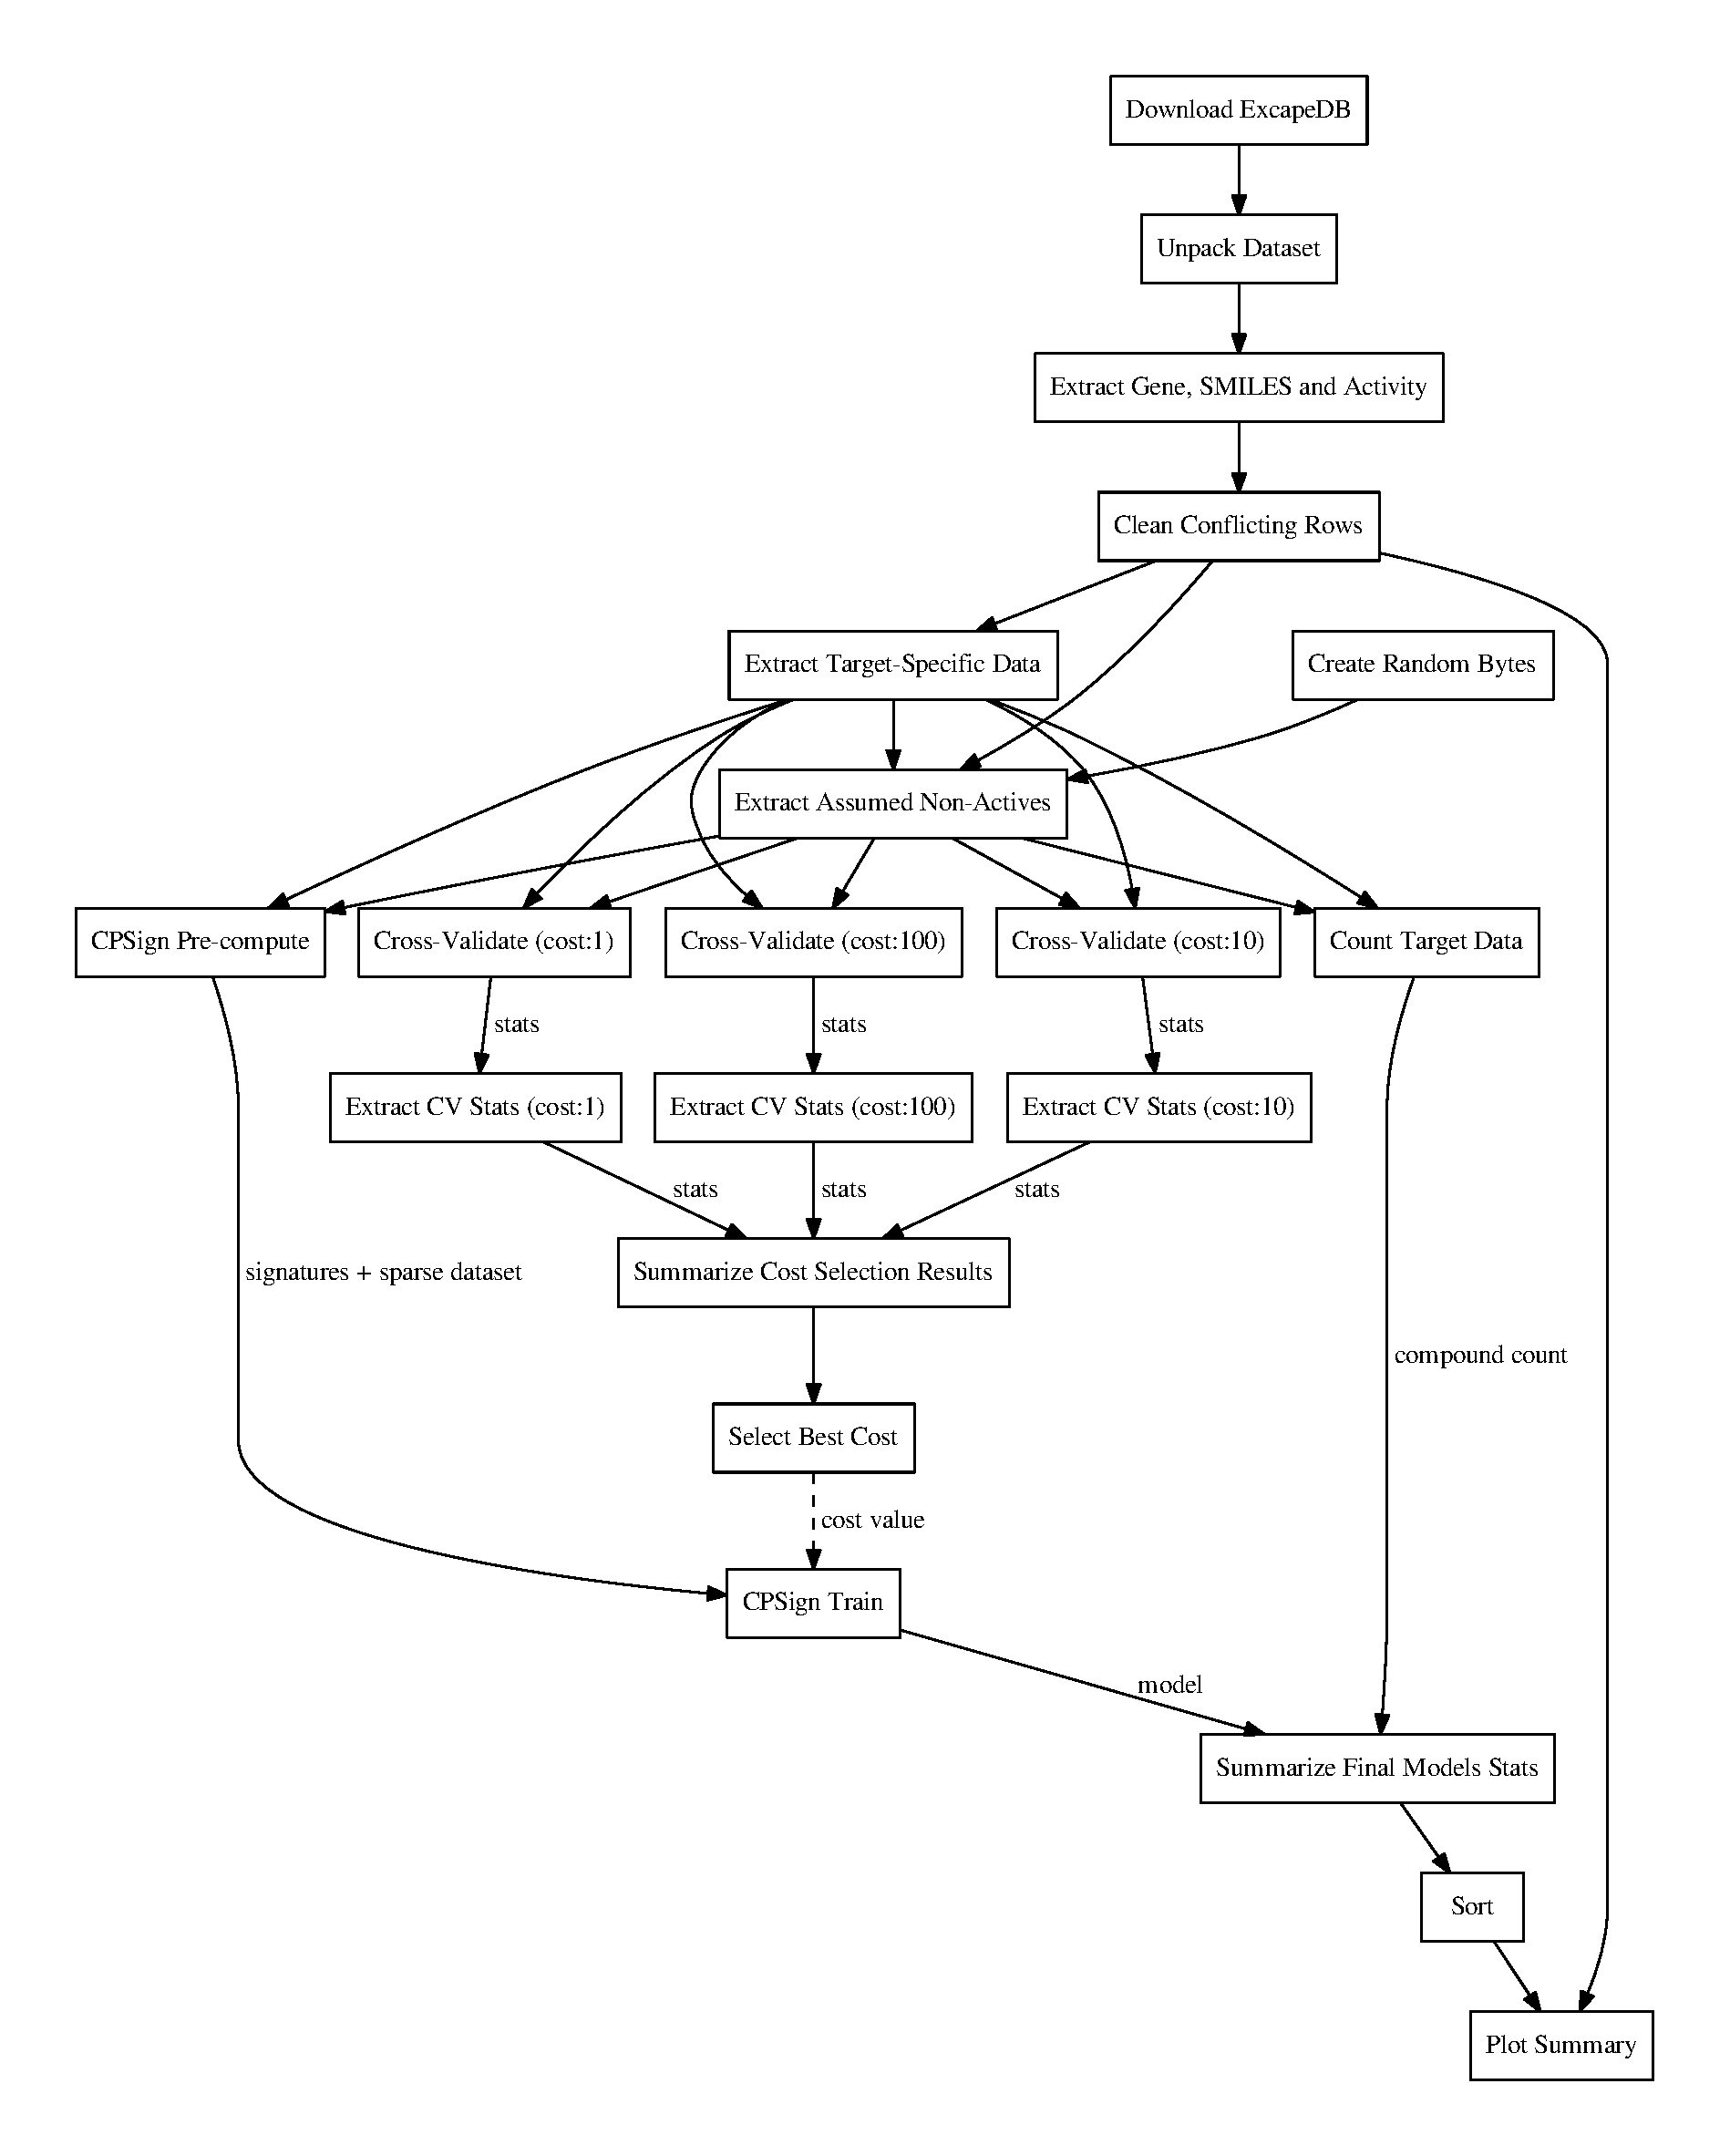
\includegraphics[width=\textwidth]{figures/workflow_graph_clean.pdf}
    \caption{Simplified directed graph of processes in the the modeling workflow used
    in the experiments in this study. Each experiment contains additions and modifications
    to the workflow, but the workflow shown here, exemplifies the basic structure,
    common among most of the workflows. For more detailed workflow
    plots, see the supplemental material.}
    \label{fig:workflow_graph_clean}
\end{figure}

\subsection*{Modeling workflow}
Before the training, the CPSign \texttt{precompute} command was run, in order to
generate a sparse representation of each target's dataset.
ACPs consisting of 10 models were then trained for each target using the CPSign software using the \texttt{train} command.
The cost value used was the one obtained from the hyperparameter tuning.
The observations added as `assumed non-actives' were not included in the calibration set to avoid biasing the evaluation.
% (See \href{https://github.com/pharmbio/ptp-project/blob/c529cf307593c40e7f822a92b224036894c95de1/exp/20180426-wo-drugbank/wo_drugbank_wf.go#L69-L101}{here}).
The computational workflows for orchestrating the extraction of data, model building,
and the collection of results for summarization and plotting were
implemented in the Go programming language using the SciPipe workflow library
that is available as open source software at
\href{http://scipipe.org}{scipipe.org} or \href{https://github.com/scipipe/scipipe}{github.com/scipipe/scipipe}.
The cost values for each target is stored in the workflow code, available on
GitHub (https://github.com/pharmbio/ptp-project).  An example of the modeling
workflow is shown in figure \ref{fig:workflow_graph_clean}, which shows the workflow
used for comparing efficiency metrics when filling up with assumed non-actives, versus
not filling up. More detailed workflow graphs are available in the supplemental
material (figure \ref{fig:workflow_detailed_fillup_vs_not} and
\ref{fig:workflow_detailed_wo_drugbank}).





%%%%%%%
% Results  %
%%%%%%%
\section*{Results}

\subsection*{Validity of models}
To check that the conformal prediction models are valid (i.e. that they predict with
an error rate in accordance to the selected significance setting), calibration plots
were generated in the cross validation step of the workflow. Three example
plots, for three representative targets (the smallest, the median-sized and the
largest, in terms of compounds in ExcapeDB) can be seen in figure
\ref{fig:calplots}, while calibration plots for all targets can be
found in the supplemental material (figure~\ref{fig:calplot_all}).
From these calibration plots we conclude that all models produce valid results over all
significance levels.

\begin{figure}[h!]
    \begin{minipage}[c]{0.3\textwidth}
        \setcounter{subfigure}{0} % Ensures that subfigures are labeled from a, b, c...
        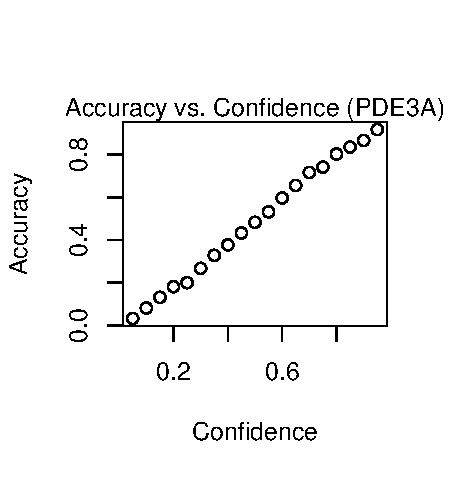
\includegraphics[width=\textwidth]{figures/calibration_plots/pde3a_calib.pdf}
        \label{fig:calplots:a}
        \subcaption{}
    \end{minipage}
    \begin{minipage}[c]{0.3\textwidth}
    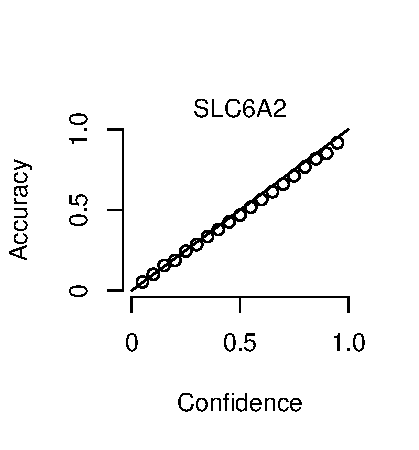
\includegraphics[width=\textwidth]{figures/calibration_plots/slc6a2_calib.pdf}
        \label{fig:calplots:b}
        \subcaption{}
    \end{minipage}
    \begin{minipage}[c]{0.3\textwidth}
        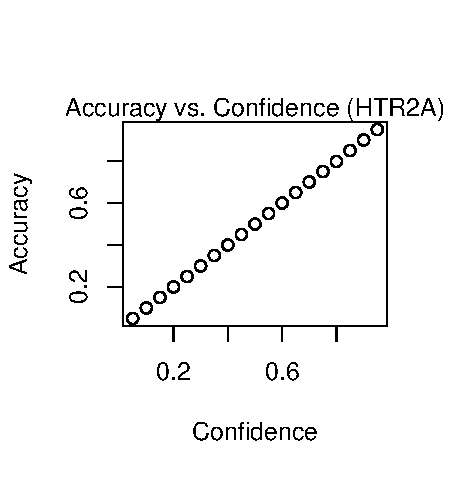
\includegraphics[width=\textwidth]{figures/calibration_plots/htr2a_calib.pdf}
        \label{fig:calplots:c}
        \subcaption{}
    \end{minipage}
    \caption{Three representative calibration plots, for models PDE3A (\ref{fig:calplots}a), SLC6A2  (\ref{fig:calplots}b),
    and HTR2A (\ref{fig:calplots}c), based on the smallest, the median, and the largest data sets in
    terms of total number of compounds. The plots show accuracy versus
    confidence, for confidence values 0.05 to 0.95 with a step size of 0.05.}
    \label{fig:calplots}
\end{figure}

\inlinetodo{Ola does not like the term 'fill up', it sounds non-scientific. Can we not simply say adding
assumed non-actives?}

%\subsection*{Before and after fill up with assumed non-actives}
\subsection*{Efficiency of models}
The efficiency metric CAOF for Dataset2 (without adding assumed non-actives)
are shown in figure~\ref{fig:21small_orig}. In figure \ref{fig:21small_fill},
the same metrics are shown for when all target datasets (still in Dataset2)
have been filled up with assumed non-actives, to compensate these target
datasets' imbalanced nature.
%, after fillup with assumed non-actives for the 21 targets with less than
%10\,000 non-actives in ExcapeDB.
We observe that by adding assumed non-actives for small, imbalanced datasets we
improve the efficiency of models trained on these datasets (OF, and CAOF, shown
by the green and blue lines respectively, improve). Thus, this strategy of
filling up the ``small'' target datasets in Dataset2 was chosen for the
subsequent analysis workflows.

\begin{figure}[h!]
    \begin{minipage}[t]{0.62\textwidth}
        \setcounter{subfigure}{0} % Ensures that subfigures are labeled from a, b, c...
        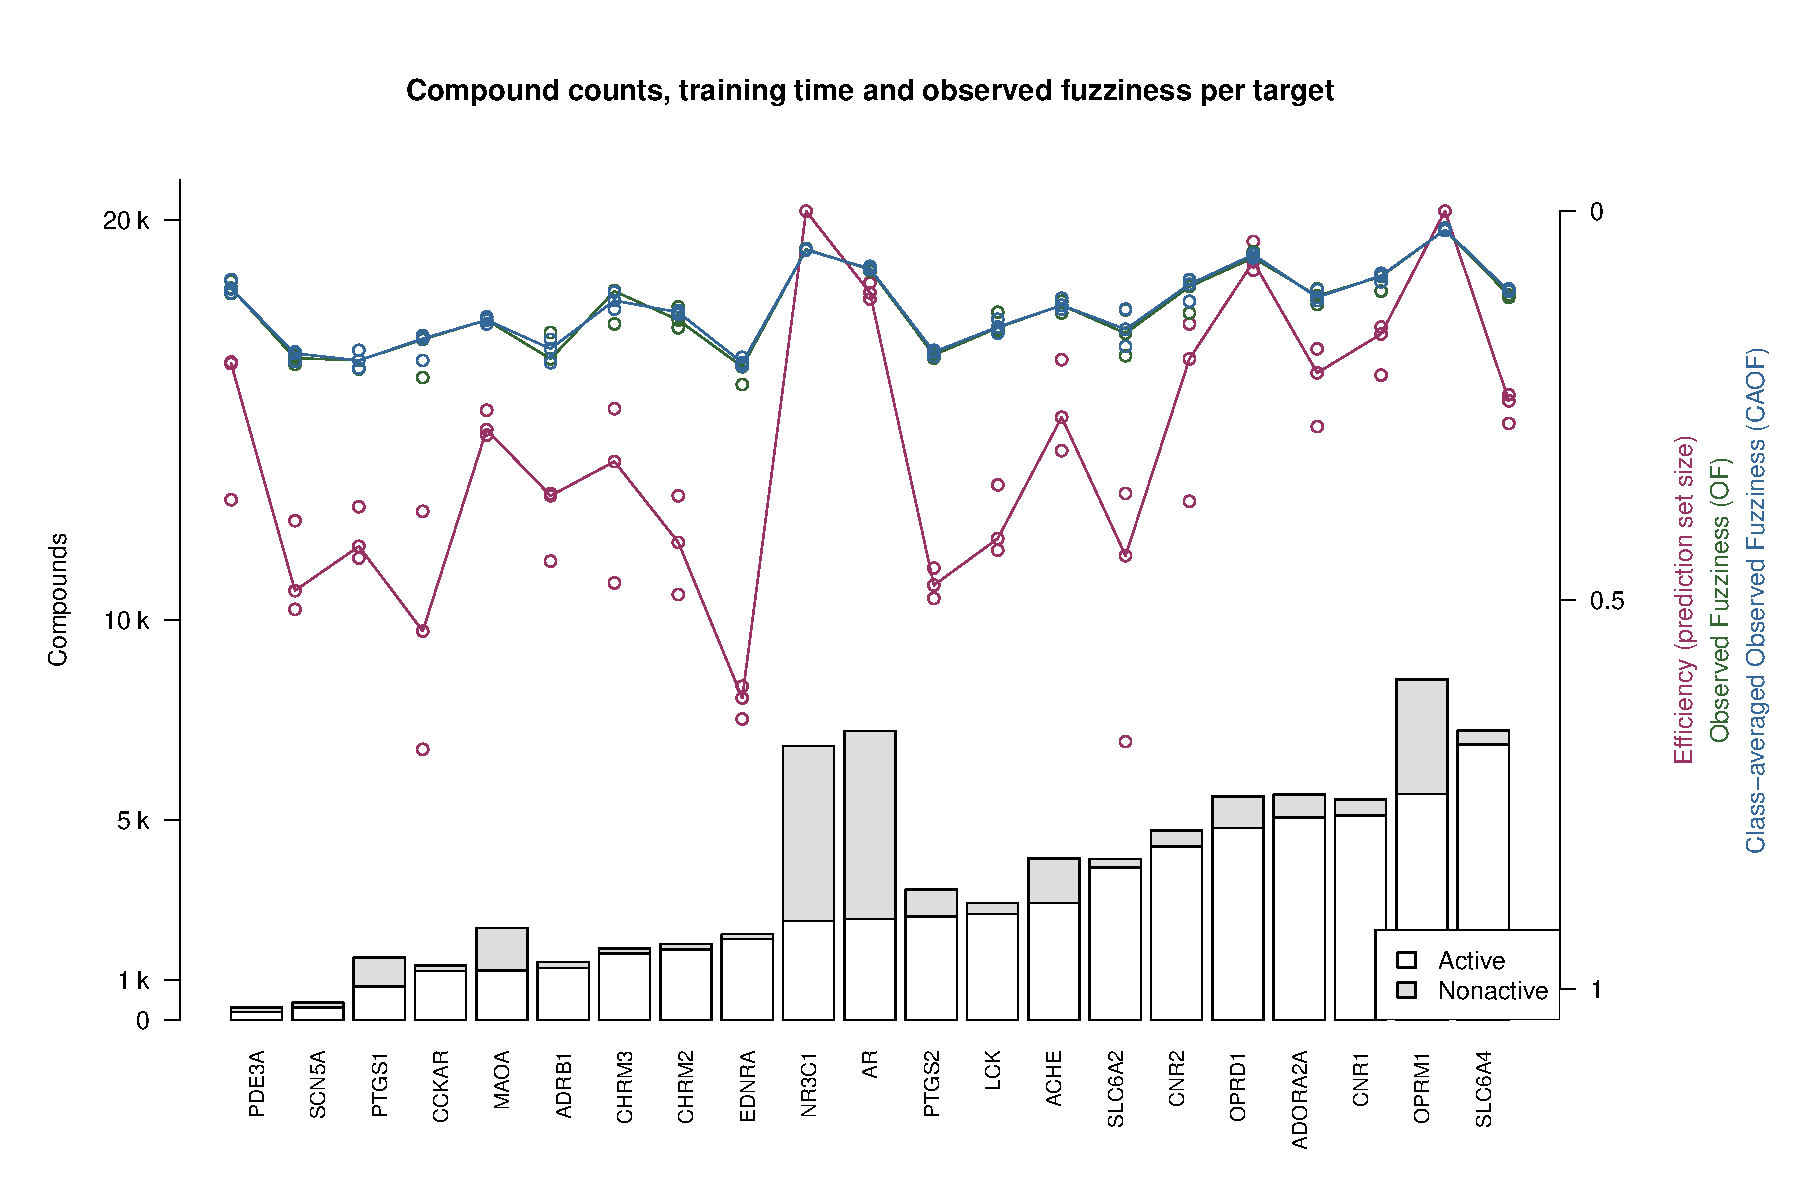
\includegraphics[width=\textwidth]{figures/21small_orig.pdf}
        \subcaption{Dataset2 without fill up of assumed non-actives.
            Circles show individual results from the three replicate runs that were
            run, while the lines show the median value from the individual replicate
            results. Targets are here sorted by number of active compounds.}
        \label{fig:21small_orig}
    \end{minipage} \\
    \begin{minipage}[t]{0.62\textwidth}
        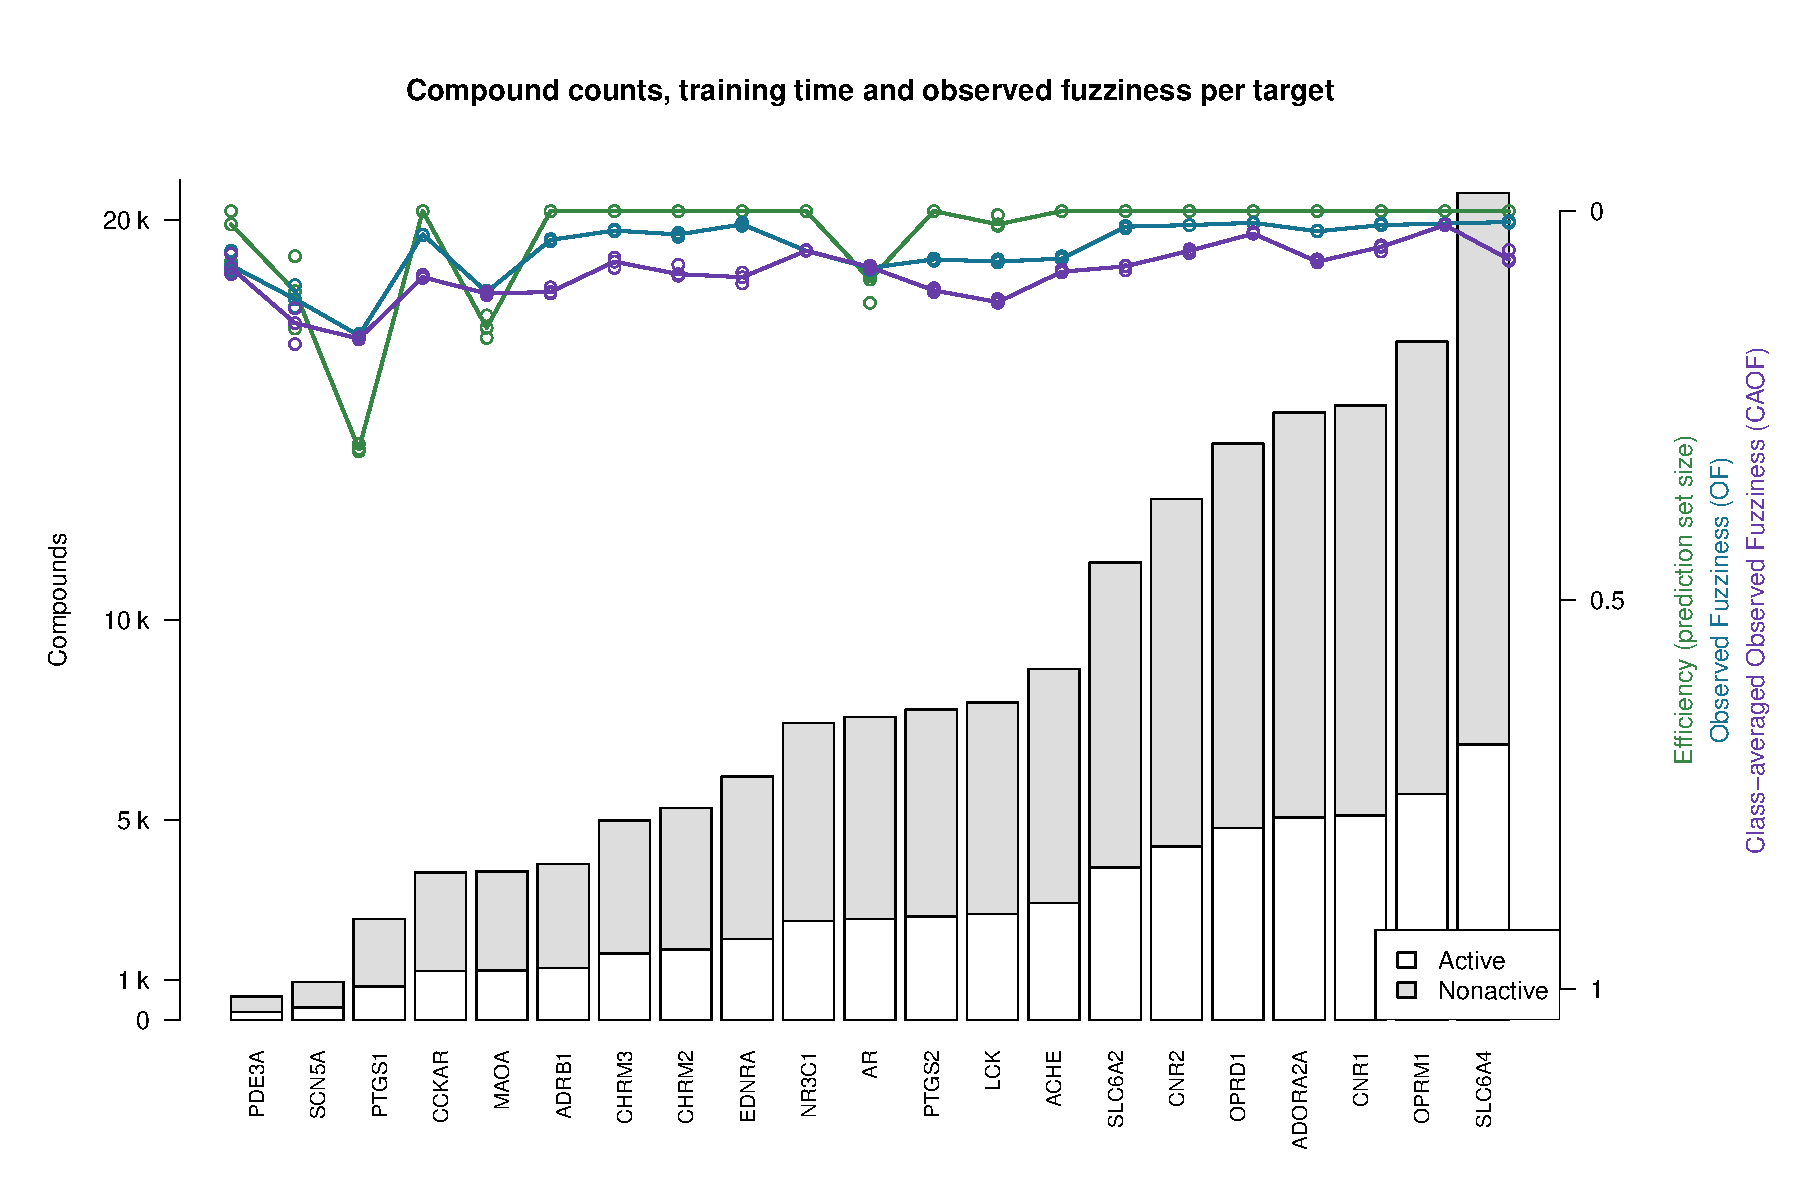
\includegraphics[width=\textwidth]{figures/21small_fill.pdf}
        \subcaption{Dataset2 after fill up with assumed non-actives.
            Circles show individual results from the three replicate runs that were
            run, while the lines show the median value from the individual replicate
            results. Targets are here sorted by number of active compounds.}
        \label{fig:21small_fill}
    \end{minipage}
    \begin{minipage}[t]{0.38\textwidth}
        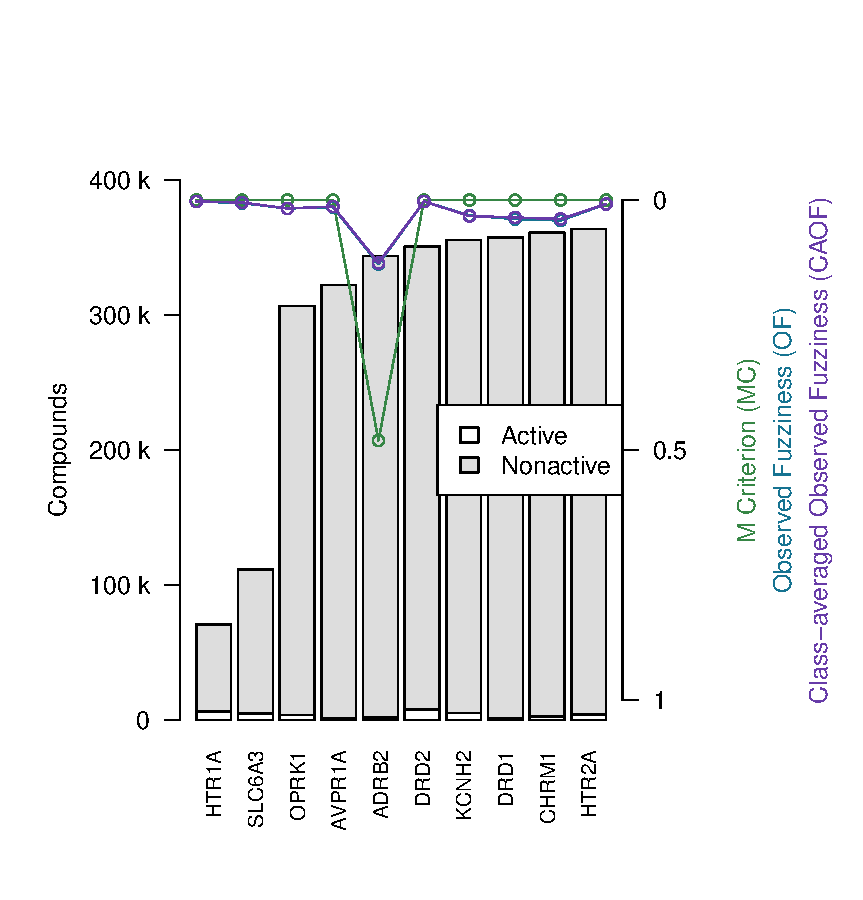
\includegraphics[width=\textwidth]{figures/10large.pdf}
        \subcaption{Dataset3, the 10 largest target datasets.
        These were not filled up with assumed non-actives.
        Targets are here sorted by total number of compounds.}
        \label{fig:10large}
    \end{minipage}
    \caption{Efficiency metrics for Dataset1 (Efficiency, Observed Fuzziness
    and Class-Averaged Observed Fuzziness) for Dataset2 and Dataset3.}
\end{figure}

%\subsection*{Efficiency}
%
%In figure \ref{fig:allmodels}, efficiency metrics Observed Fuzziness (OF), Class-Averaged OF
%(CAOF) for each model is , training time and validation.
%\inlinetodo{What can be seen from the figures?}
%
%\begin{figure}[h!]
%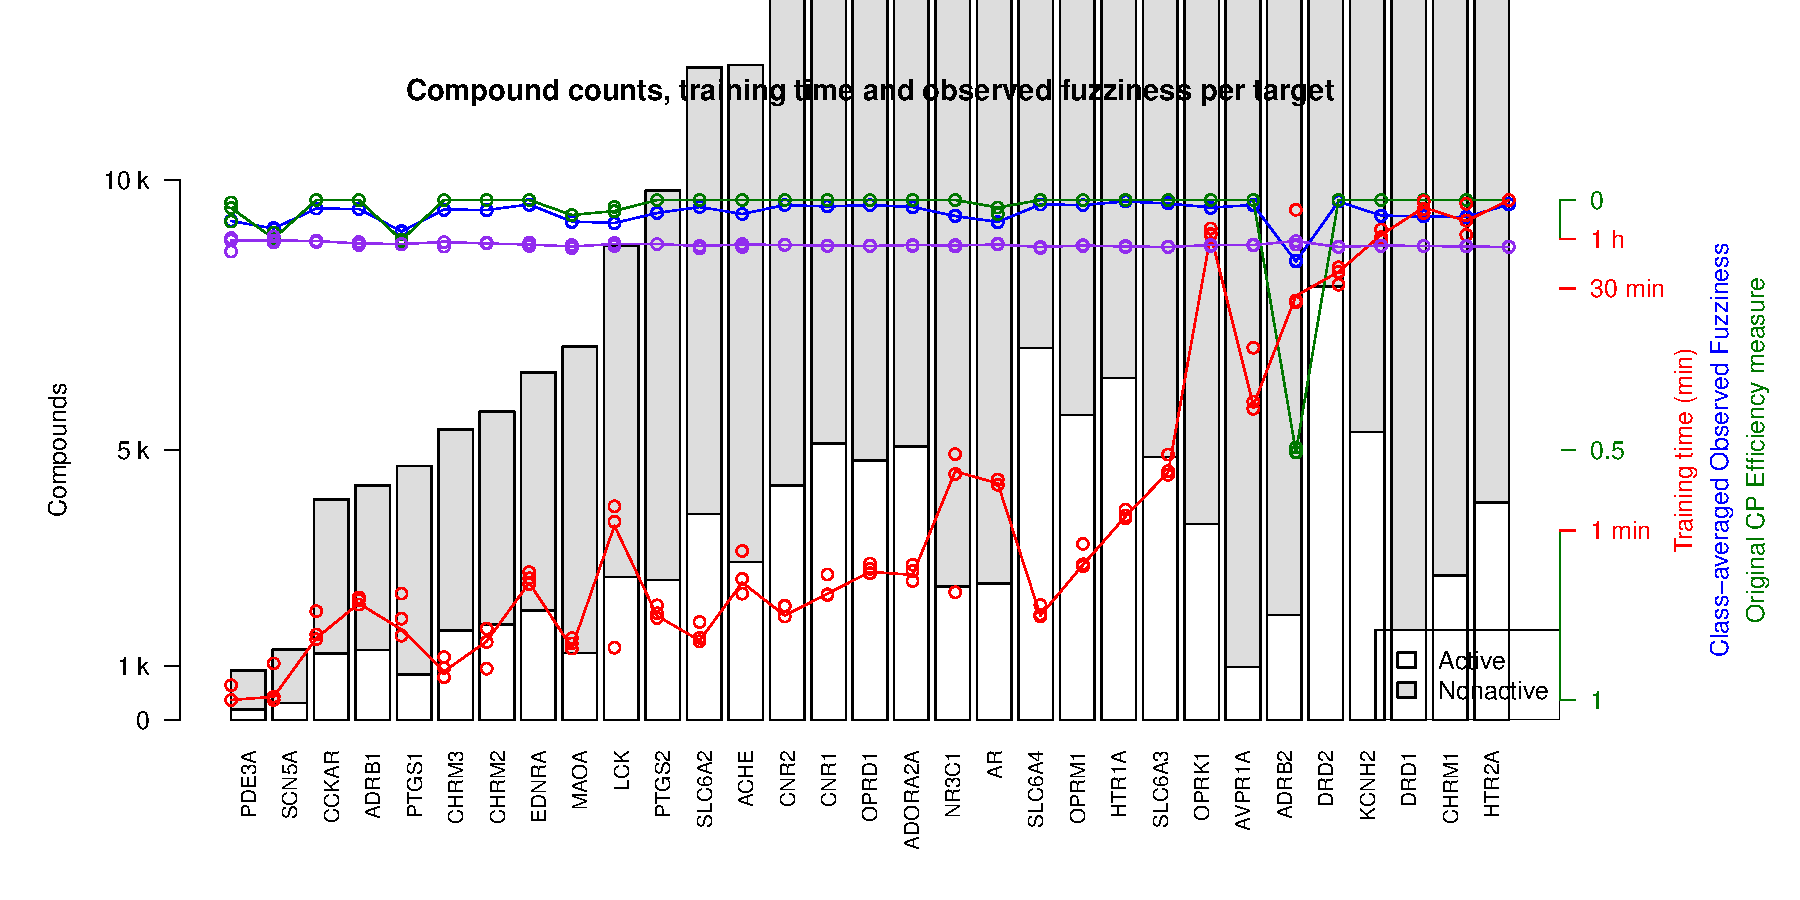
\includegraphics[width=\textwidth]{figures/allmodels_wo_drugbank.pdf}
%    \caption{All models with the smaller ones being filled up with assumed non-actives.}
%    \inlinetodo{Extend the figure caption!}
%    \label{fig:allmodels}
%\end{figure}

\subsection*{External validation}

In order to validate the predictive ability of the trained models, a new
dataset was created (Dataset4)\todo{Create a table with the three Datasets and
how they differ} by withholding 1\,000 compounds from the ExcapeDB dataset, to
form an external validation dataset. The compounds chosen to be withheld were
the following: i) all small molecules in DrugBank (version 5.0.11) with status
``withdrawn'', for which we could find either a pubchem ID or a CHEMBL ID, ii)
a randomly selected subset of the remaining compounds in DrugBank 5.0.11, with
status ``approved'', for which we could also find PubChem or CHEMBL IDs, until
a total number of 1\,000 compounds was reached.  No regard was paid to other
drug statuses in DrugBank such as ``investigational''.

The models built were validated by predicting the binding activity against each
of the 31 targets for all compounds for which we had known binding data for a
particular target. The validation was done with CPSign's \texttt{validate}
command, predicting values at confidence levels 0.8 and 0.9.
%
In figure \ref{fig:valplots} predicted versus observed labels for Dataset4,
for confidence levels 0.8 and 0.9 respectively is shown. We see how the number
of prediction of ``both'' labels increase when the confidence level increases
from 0.8 to 0.9. This is as expected, as this means that fewer compounds could
be predicted to only one specific label with the higher confidence level. The number of
``Null'' predictions decreases at a higher confidence, which is expected as the
predictor must accept less probable (in the Conformal Prediction ranking sense)
predictions to be considered part of the prediction region at a higher confidence.
This behaviour might seem backwards, but at a higher confidence the predictor
has to include less likely predictions for it to reach the specified confidence
level, which leads to larger prediction sets.

\begin{figure}[h!]
\begin{minipage}[c]{0.38\textwidth}
    \setcounter{subfigure}{0} % Ensures that subfigures are labeled from a, b, c...
    \subcaption[Predicted versus observed labels, for all targets at confidence level 0.8]{
    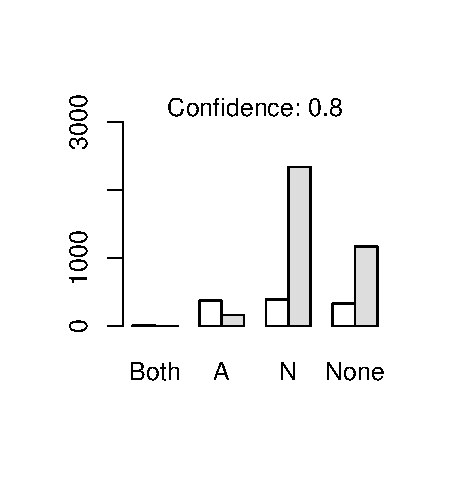
\includegraphics[width=1\textwidth]{figures/validation_plots/alltargets_0p8_valplot.pdf}
    }\label{fig:valplots:a}
\end{minipage}
\hspace{0.10\textwidth}
\begin{minipage}[c]{0.38\textwidth}
    \subcaption[Predicted versus observed labels, for all targets at confidence level 0.9]{
        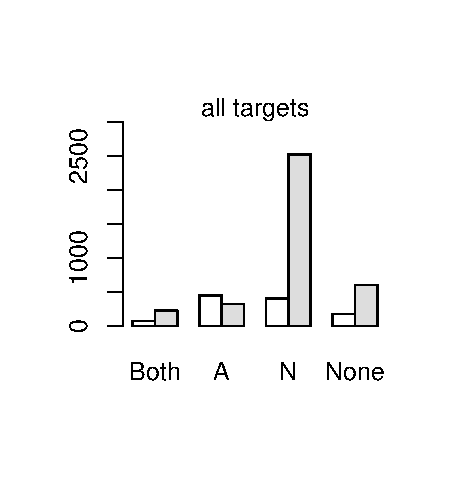
\includegraphics[width=1\textwidth]{figures/validation_plots/alltargets_0p9_valplot.pdf}
    }\label{fig:valplots:b}
\end{minipage}
    \caption{Predicted versus observed labels, for all targets, for the prediction data,
    at confidence level 0.8 (\ref{fig:valplots:a}) and 0.9
    (\ref{fig:valplots:b}).  The labels on the X-axis indicate predicted labels
    (Null, Active (A), Non-active (N) or Both). White in the stacked bar plot
    means that the observed label was Active (A), while grey means the observed
    label was Non-Active (N).
    }
    \label{fig:valplots}
\end{figure}

\subsection*{Target Profile-as-a-Service}
All models based on Dataset2 were published as microservices with REST APIs
publicly made available using the OpenAPI specification on an OpenShift cluster
and a web page federating all the models were created. The OpenAPI
specification is a standardisation for how REST APIs are described, it means
that there is a common way for looking up how to use the REST API of a web
service and that greatly simplifies the process of tying multiple different web
services together. It simplifies calling the services from scripts as well as
from other web pages, such as the web page(figure~\ref{fig:web}) that makes a profile image out of
the multiple QSAR models. At the top of the web page (See figure~\ref{fig:web})
is an instance of the JSME editor~\cite{Bienfait2013} in which the user can
draw a molecule. As the user draws the molecule the web page extracts the
SMILES from the editor and sends it to the model services to make predictions
based on all available models. The user can set a threshold for the confidence
and get visual feedback on whether the models predict the drawn molecule as
active or non-active, for each of the targets, with the chosen confidence.  On the right hand is also a
graphical profile in the form of a bar plot where confidence of active is
drawn in the positive direction and confidence for non-active is the reverse
direction. Hovering it will give information about exactly which model a
certain peak in the bar charts corresponds to. The web page is accessible at
\url{http://modelingweb.service.pharmb.io/predict/profile/ptp-wo-drugbank}\todo{make
short nice URL with pharmb.io and UU logo}.
\begin{figure}
    \begin{minipage}{0.70\textwidth}
        \setcounter{subfigure}{0} % Ensures that subfigures are labeled from a, b, c...
        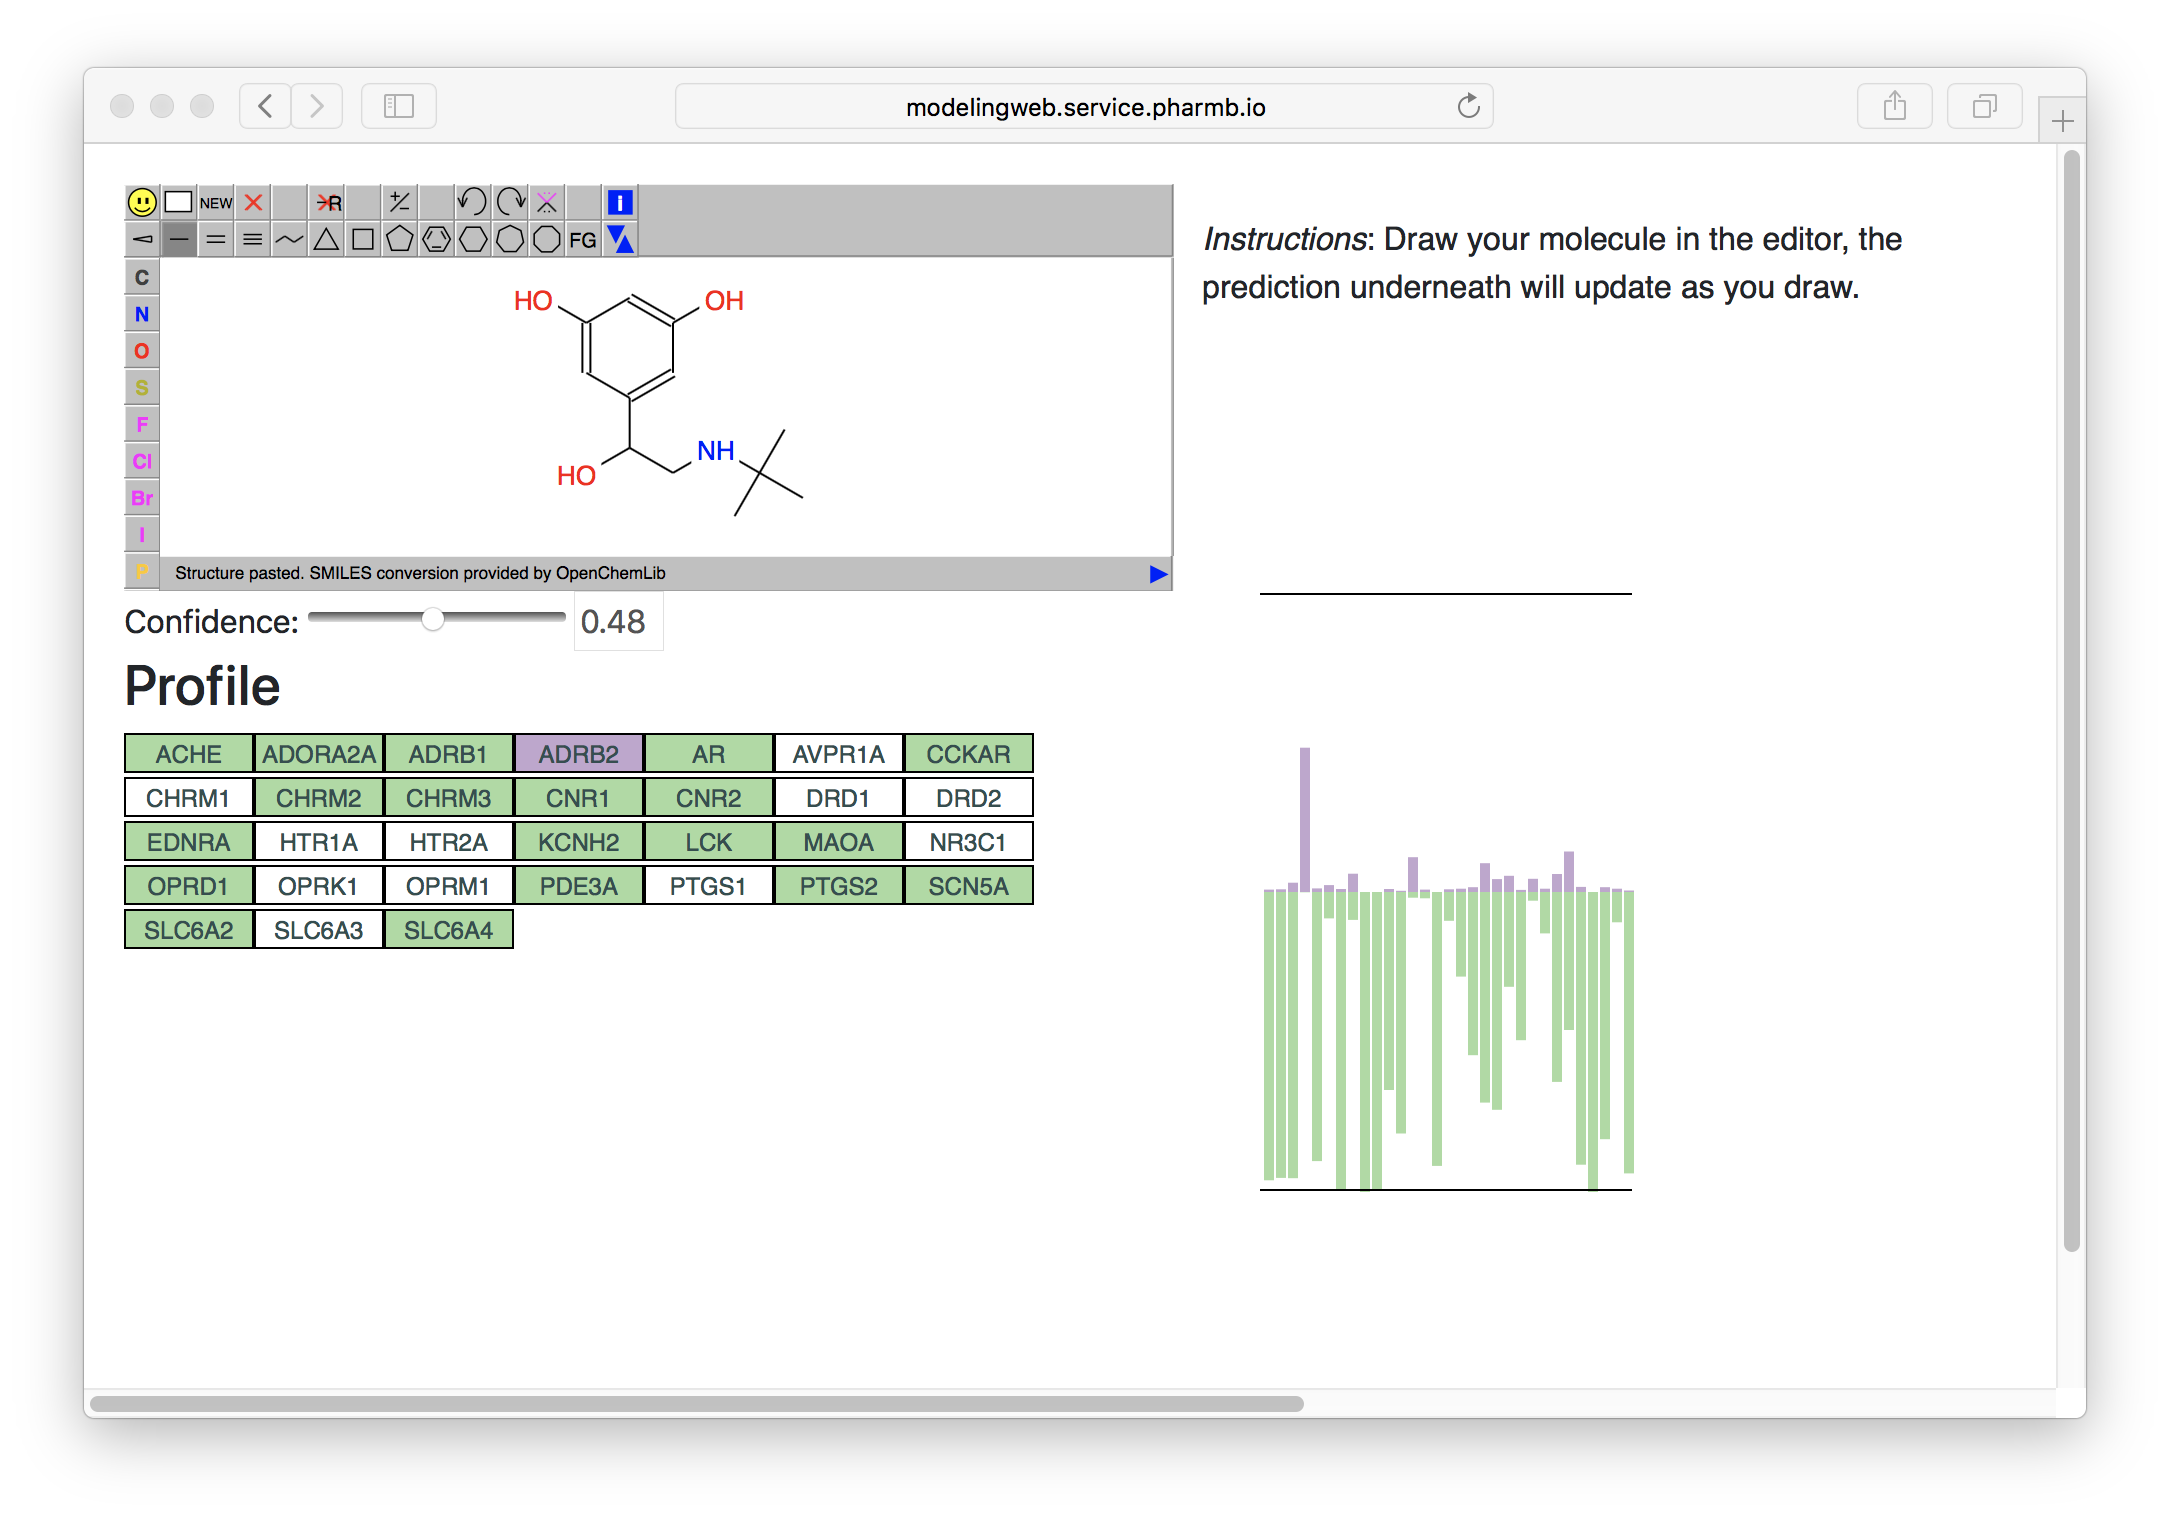
\includegraphics[height=0.37\textheight]{figures/terbutaline.png}
        \subcaption{The profile as it looks on the web page. The user draws a
        molecule, selects a confidence and then the profile updates
        underneath.}
        \label{fig:terbutaline:a}
    \end{minipage}
    \quad
    \begin{minipage}{0.25\textwidth}
        \fbox{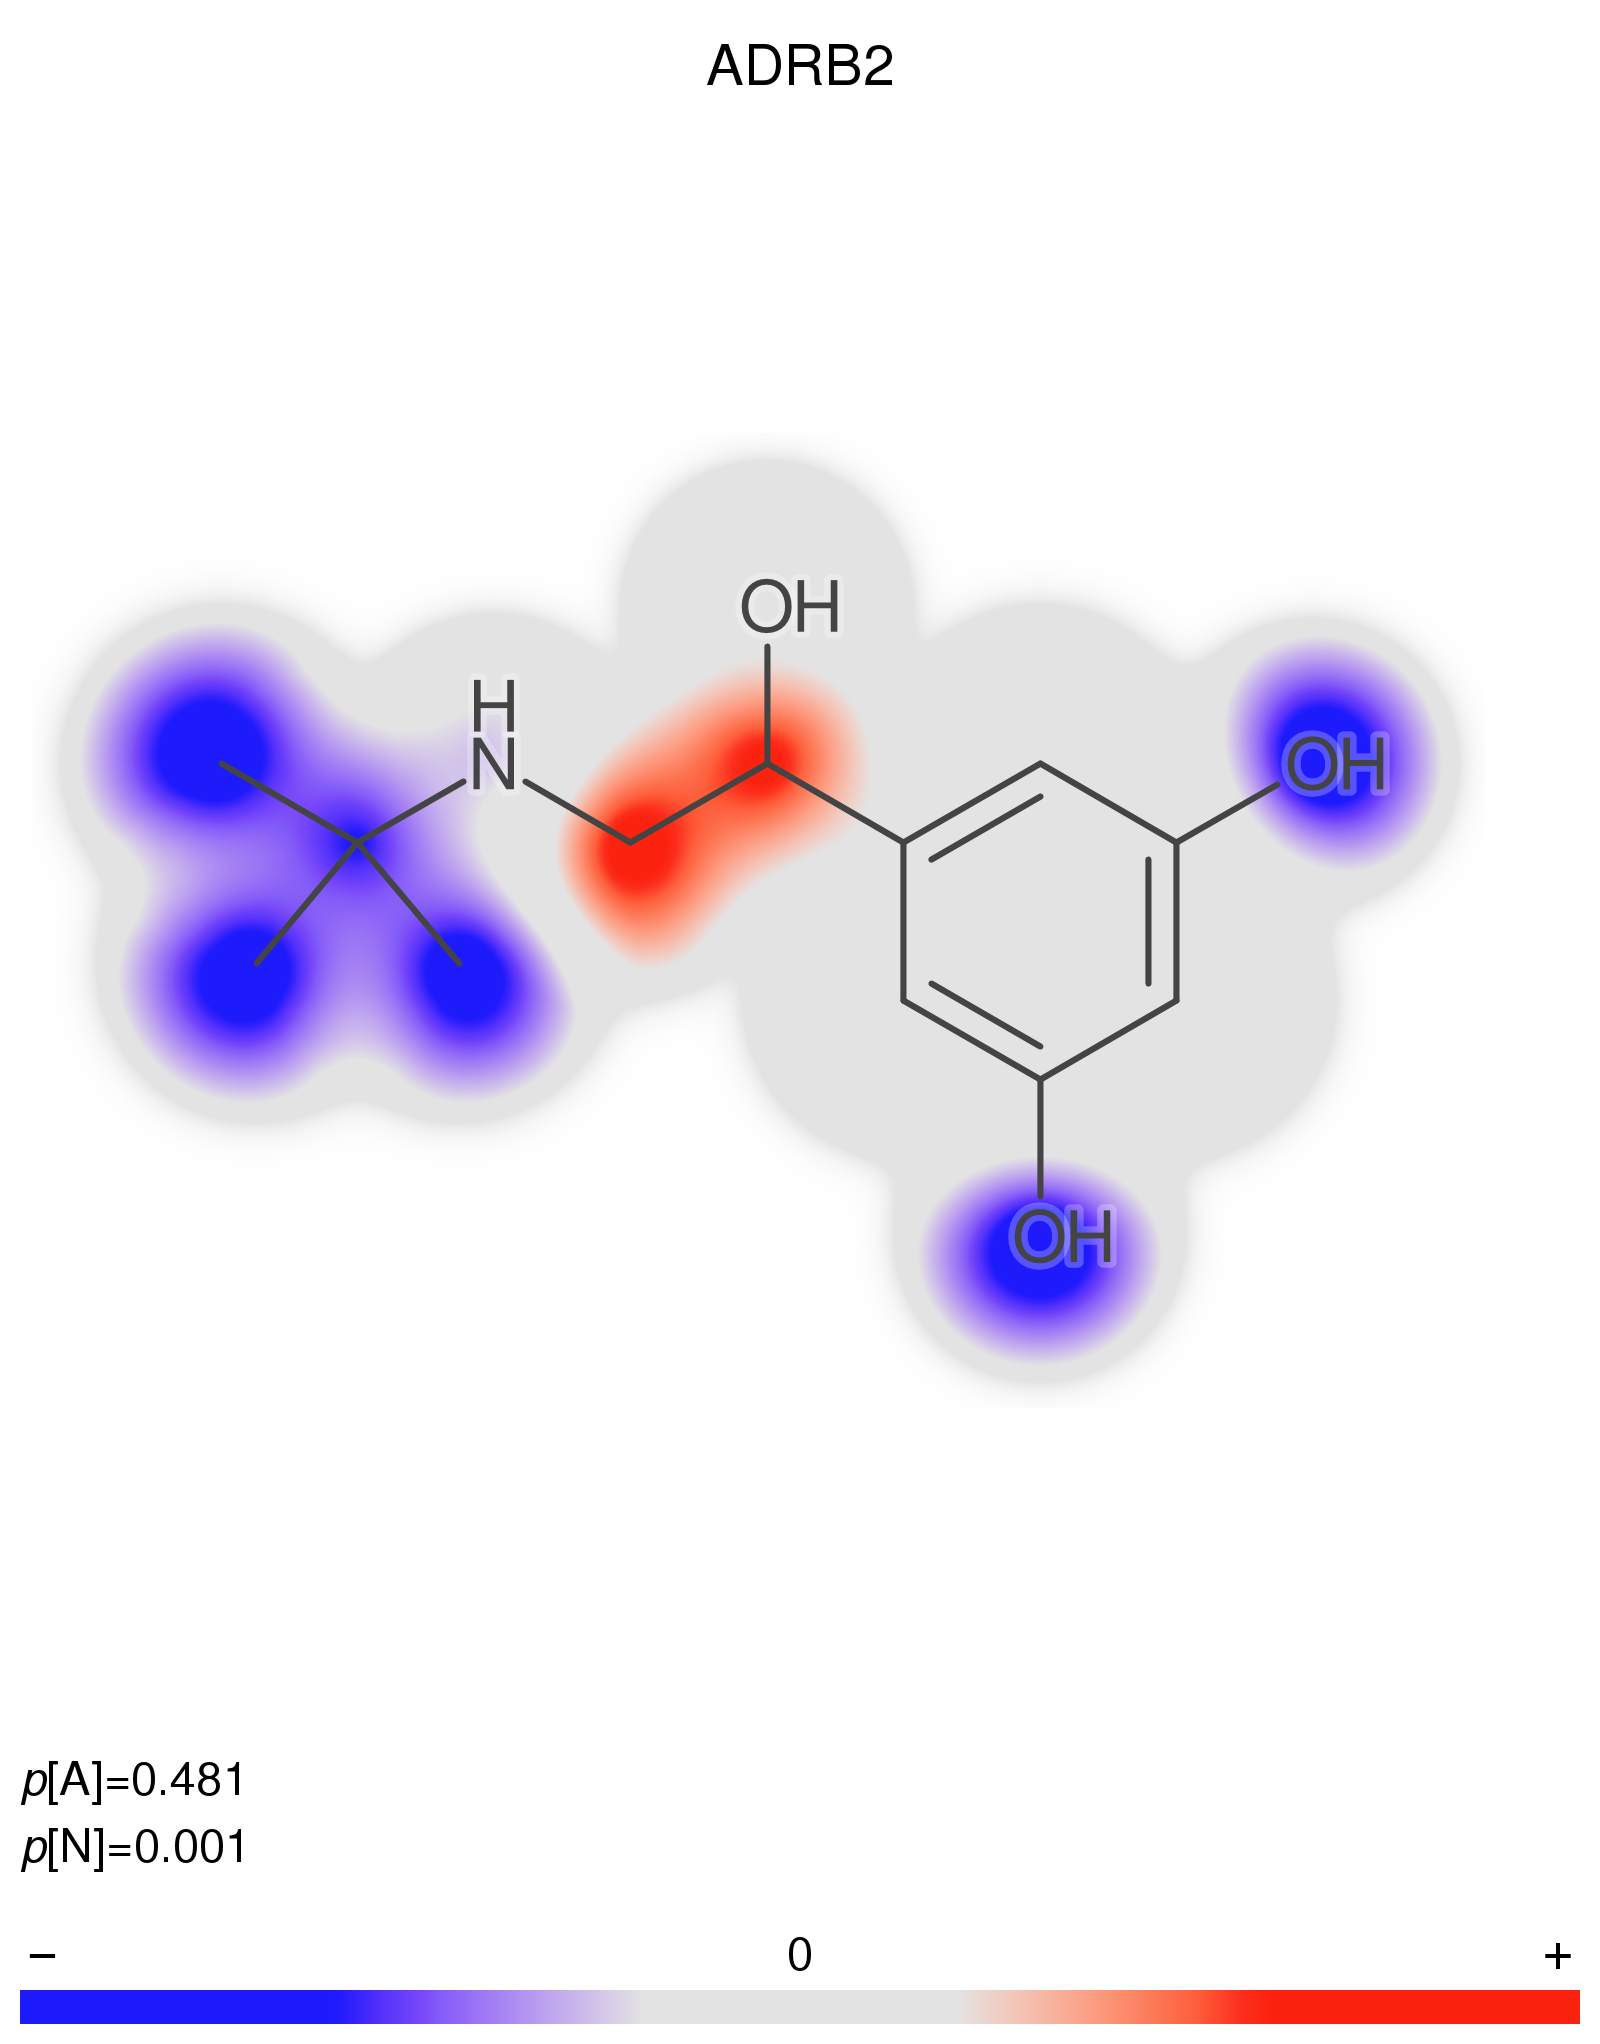
\includegraphics[height=0.23\textheight]{figures/terbutaline2.png}}
        \subcaption{Coloring of which parts of the molecule contributed the
        most to the prediction for ADBR2.}
        \label{fig:terbutaline:b}
    \end{minipage}
    \caption{The prediction profile for Terbutaline, a known selective beta-2
    adrenergic agonist  used as a broncho\-dilator and tocolytic
    \label{fig:web}}
\end{figure}

\subsection*{Example predictions}
Using the models from the external validation dataset (Dataset4), target
profiles were predicted for three molecules from the test set
(figure~\ref{fig:threeprofiles}), \textit{i.e.}, the profiles were made for
drugs that the models have not seen before. Figure~\ref{fig:threeprofiles:a}
shows the target profile for Tacrine, a centrally acting anticholinesterase,
with a distinct peak for the ACHE gene, es expected. Further, we note that most
other targets are predicted as negative with high p-values (green color) or
predicted as active with relatively low p-values (purple color).
Figure~\ref{fig:threeprofiles:b} shows the target profile for Pilocarpine, a
muscarinic acetylcholine receptor M$_1$ agonist, with a target profile
consisting of mostly negative predictions, and only mildly two active targets
(CHRM1 and LCK). Here we note that LCK has a similar p-value for active and
non-active, and for a conformal prediction the lowest p-value is sometimes
referred to as credibility - meaning that even if a prediction has a high
p-value, its credibility and hence usefulness in a decision setting might be
low. Figure~\ref{fig:threeprofiles:c} shows the target profile for Pergolide,
an agonist for DRD1, DRD2, HTR1A, and HTR2A which shows up as the four highest
positive predictions in the profile.

\begin{figure}
\hfill
\begin{minipage}[t]{0.3\textwidth}
    \setcounter{subfigure}{0} % Ensures that subfigures are labeled from a, b, c...
    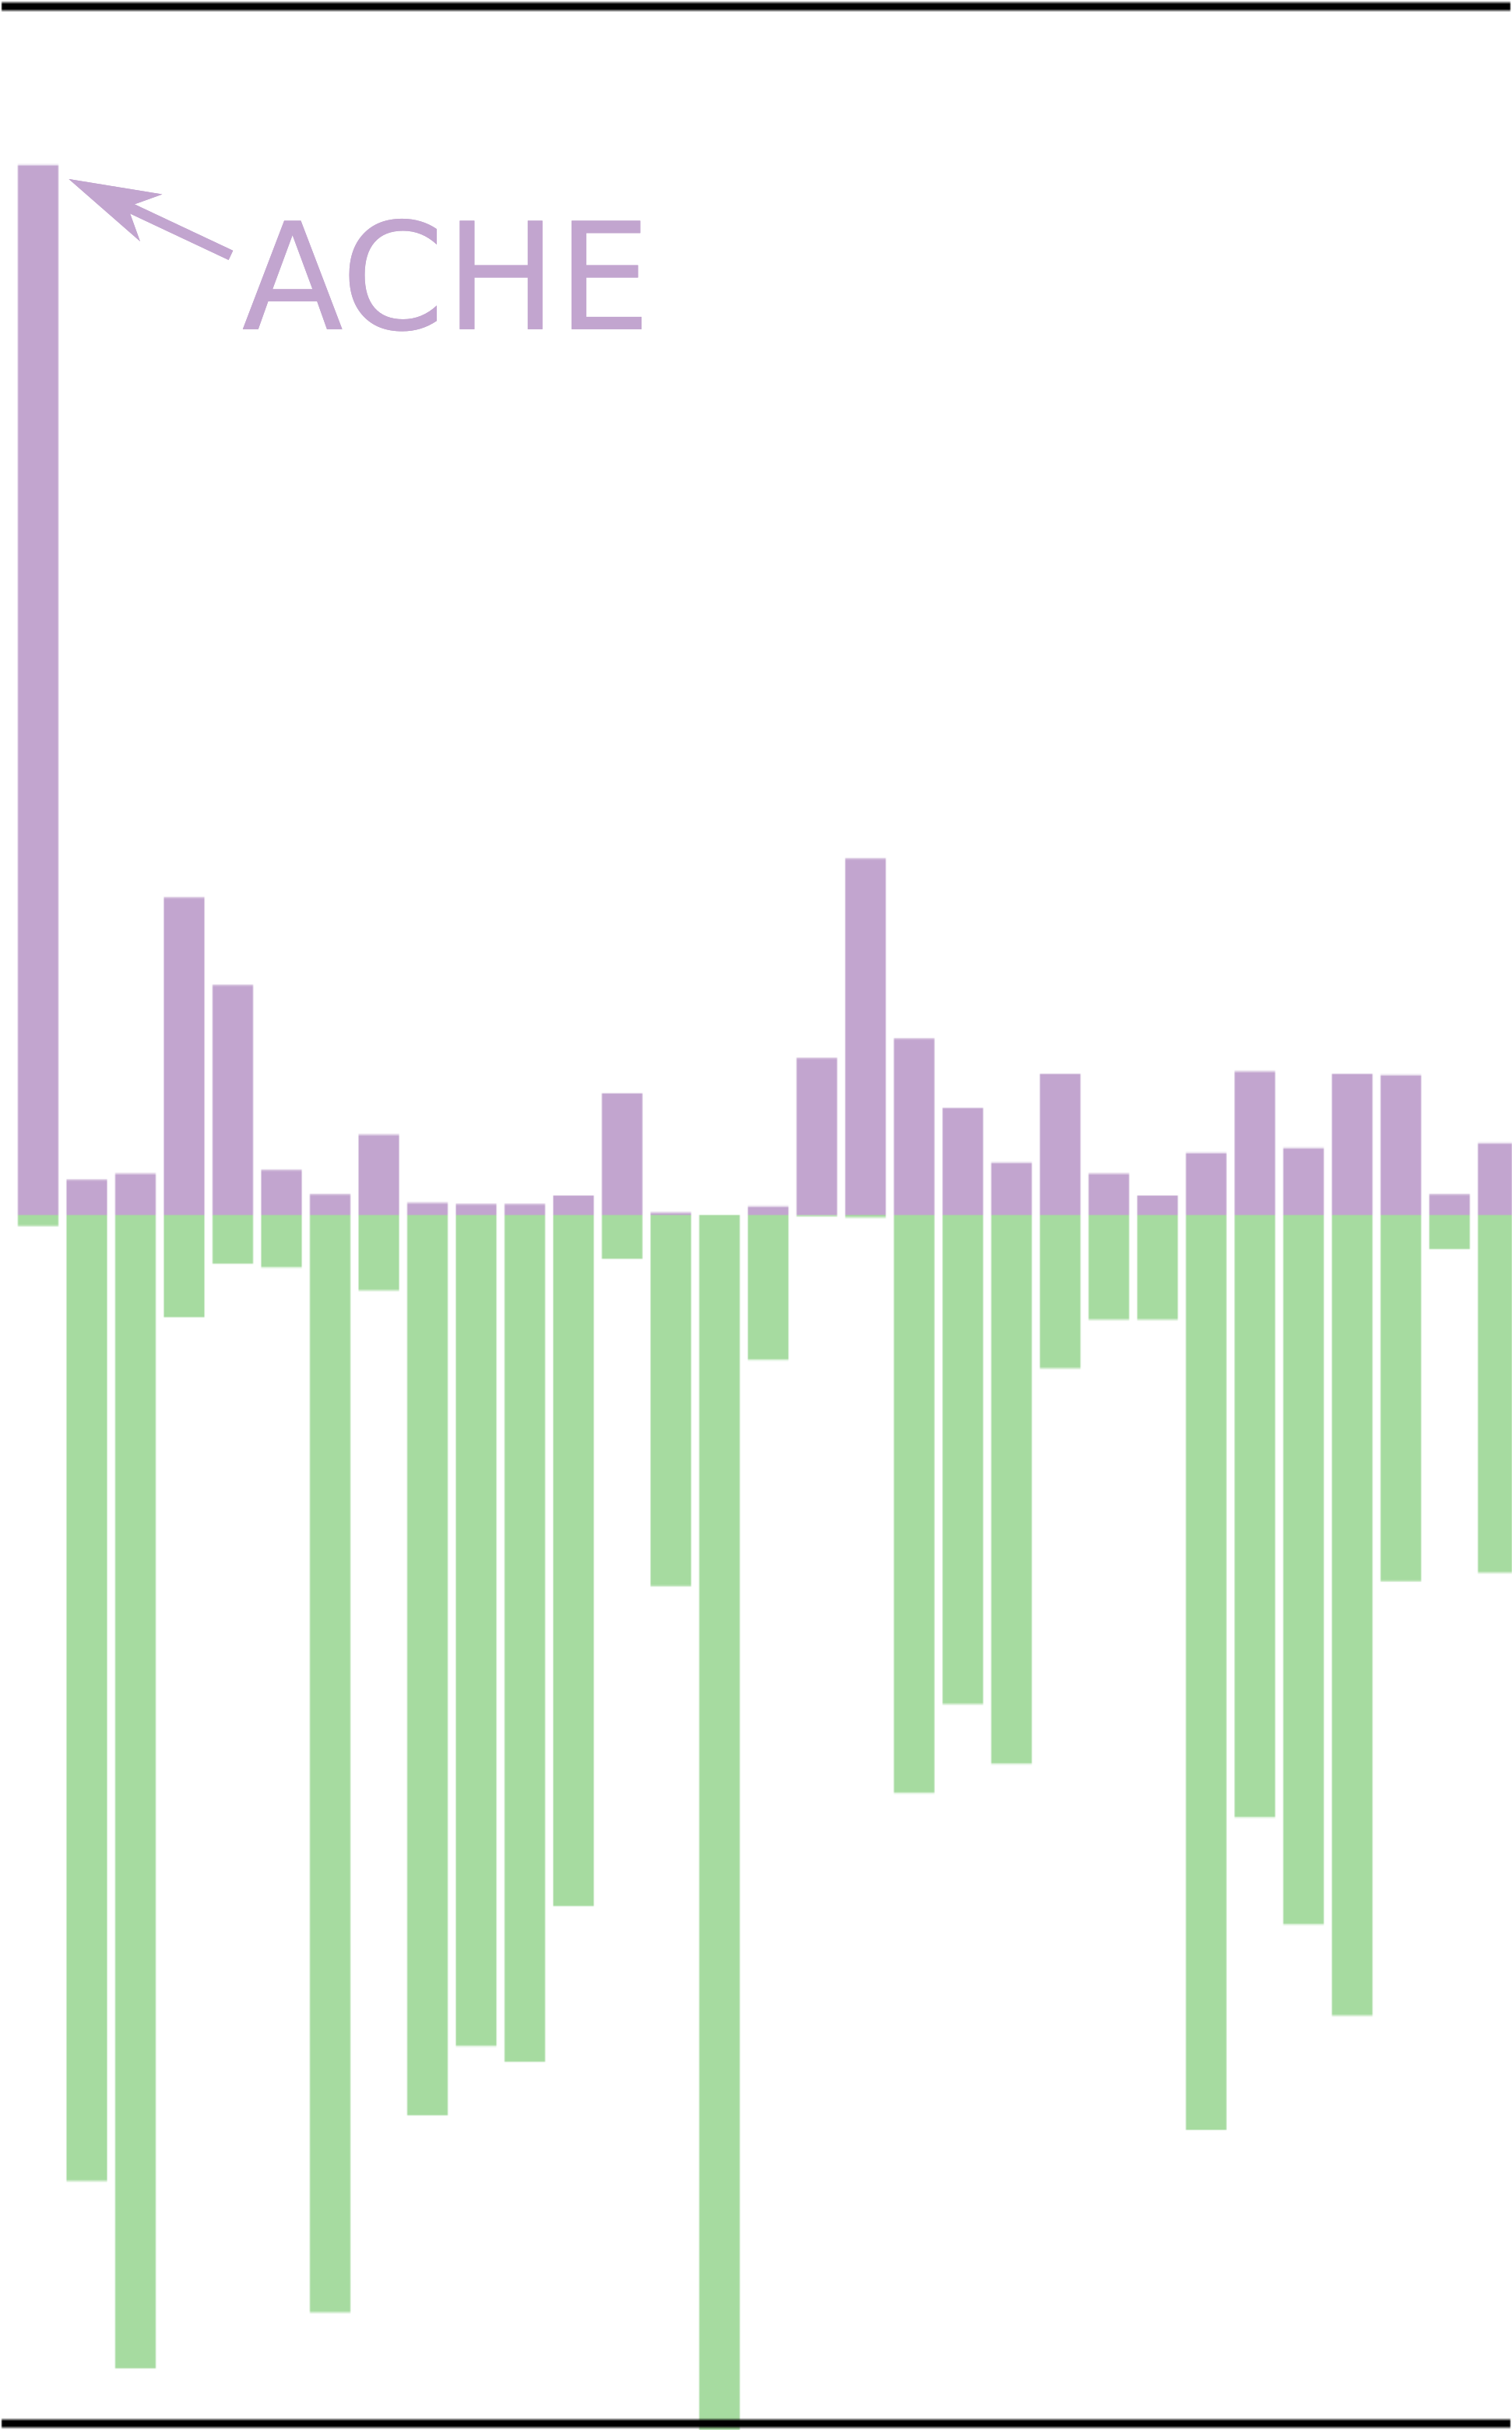
\includegraphics[width=\linewidth]{figures/chembl95.png}
    \subcaption{The profile for Tacrine, a centrally acting anticholinesterase,
    with a distinct peak for the ACHE gene.}
    \label{fig:threeprofiles:a}
\end{minipage}
\hfill
\begin{minipage}[t]{0.3\textwidth}
    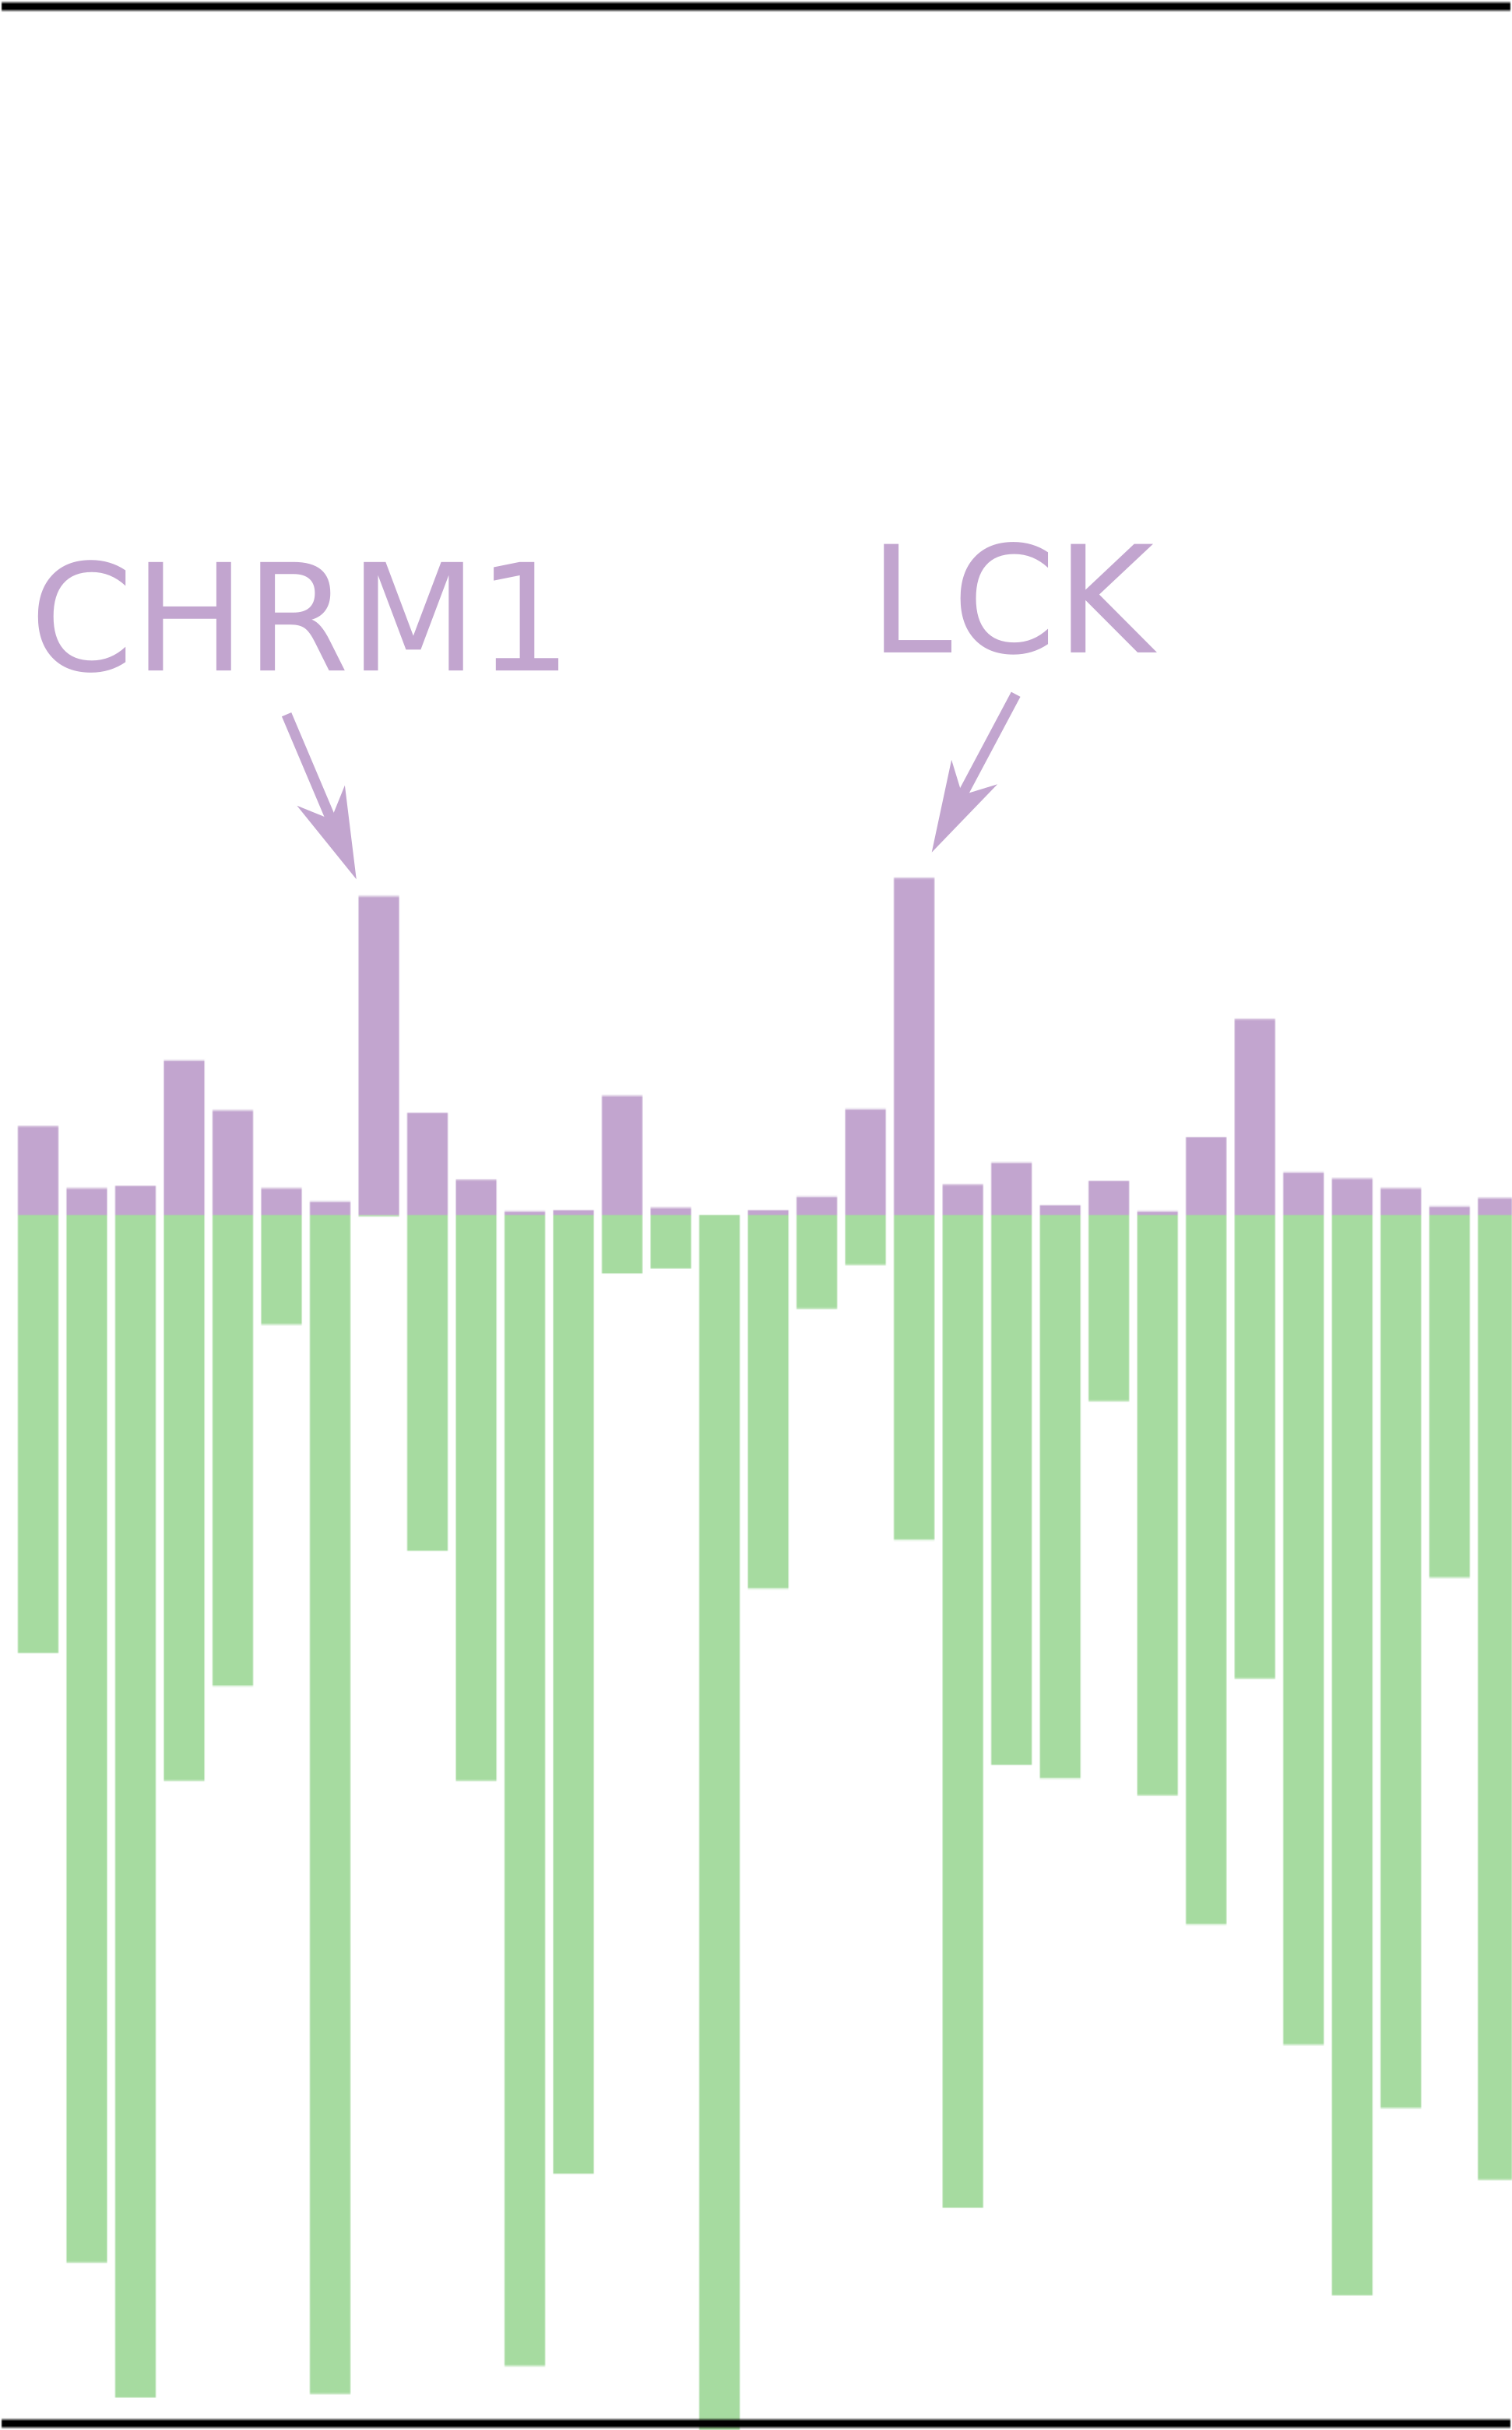
\includegraphics[width=\linewidth]{figures/chembl550.png}
    \subcaption{The profile for Pilocarpine, a muscarinic acetylcholine
    receptor M$_1$ agonist, with only two moderately higher peaks for positive
    prediction, CHRM1 and LCK.}
    \label{fig:threeprofiles:b}
\end{minipage}
\hfill
\begin{minipage}[t]{0.3\textwidth}
    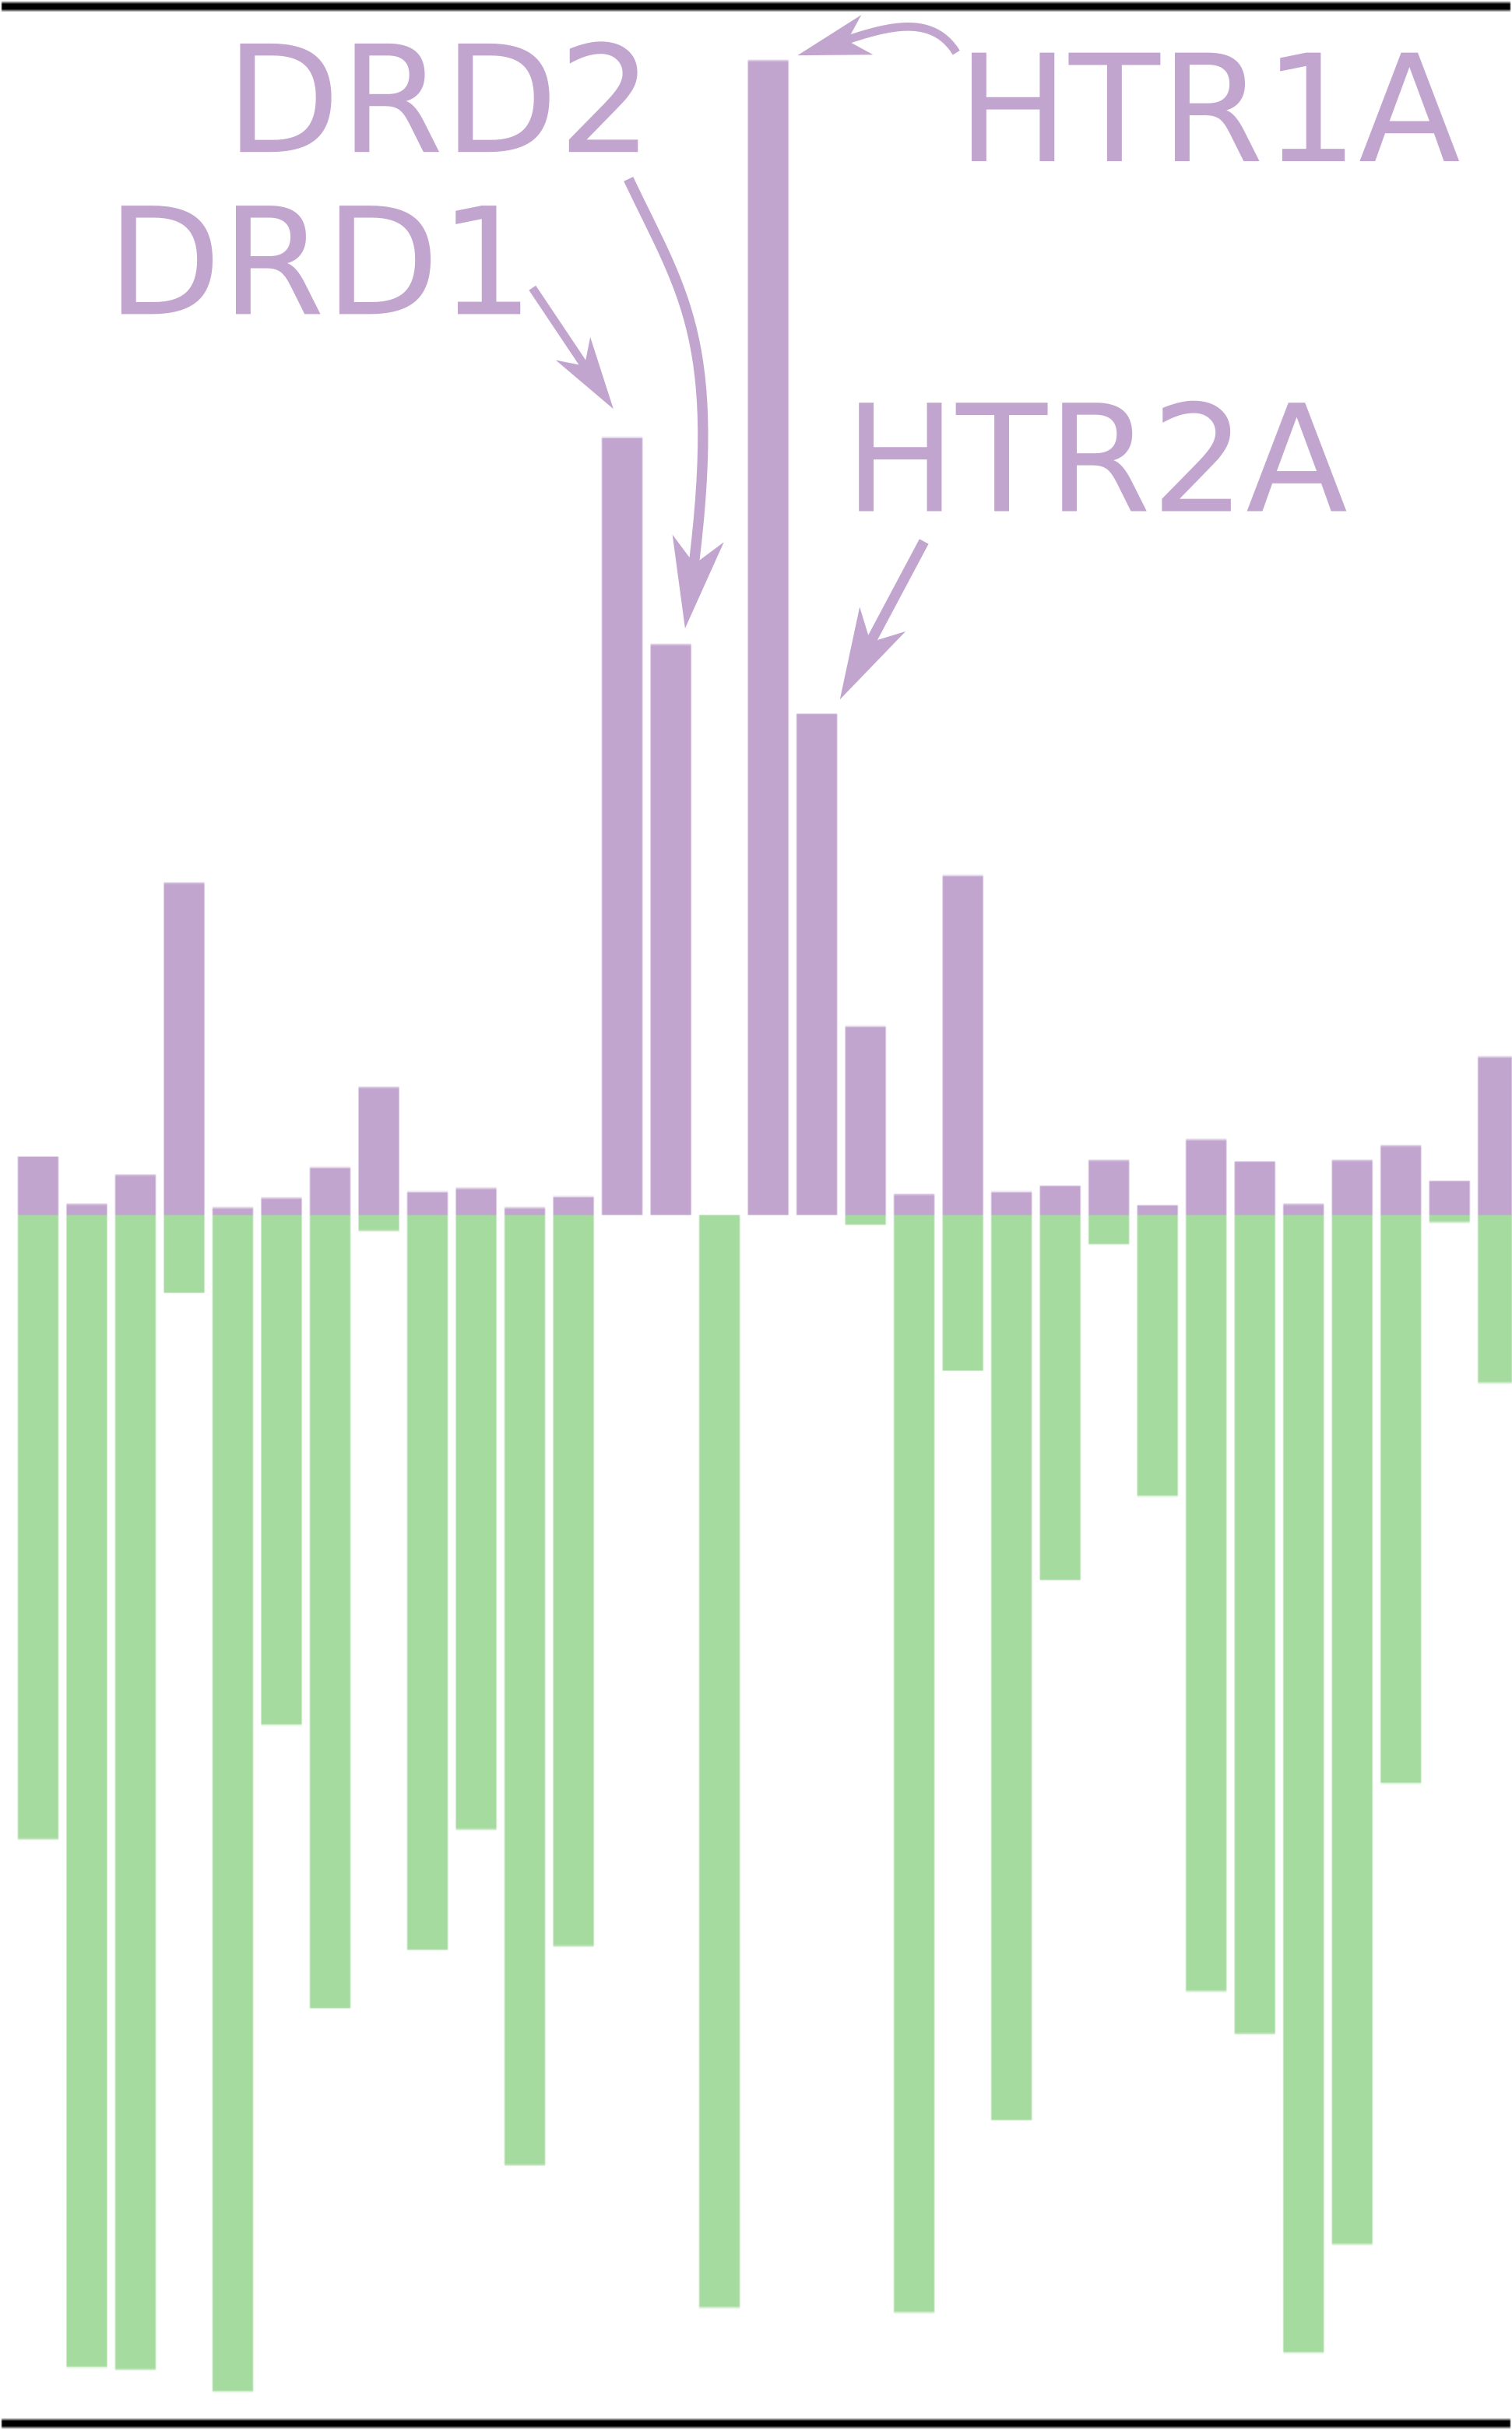
\includegraphics[width=\linewidth]{figures/chembl531.png}
    \subcaption{The profile for Pergolide, a DRD1, DRD2, HTR1A, and HTR2A
    agonist, which is reflected by the four highest p-values for a positive
    prediction.}
    \label{fig:threeprofiles:c}
\end{minipage}
\hfill
\caption{Profiles for a few of the removed drugs using the validation models,
    \textit{e.g.}, these molecules are not in the training sets for the models.
    \label{fig:threeprofiles}}
\end{figure}



%%%%%%%
% Discussion  %
%%%%%%%
\section*{Discussion}
The use of workflows to automate preprocessing and model training and make it
completely reproducible has several implications. Primarily, the entire process
can be repeated as data change, e.g. new data is made available or data is
curated. In our case, the preprocessing can be re-run when a new version of
ExCAPE-DB is released, and new models trained on up-to-date data can be
deployed and published without delay. The components of the preprocessing
workflow are however general, and can be re-used in other settings as well.
Further, a user can select the specific targets that will be preprocessed, and
focus the analysis on smaller subsets without having to preprocess and train
models on all targets which could be resource-demanding. With a modular
workflow it is also easy to replace specific components, such as evaluating
different strategies and modeling methods.

The packaging of models as docker containers makes them portable, to be
transferred and deployed on different systems, including servers or laptops on
public and private networks without cumbersome dependency management. We chose
to deploy our services inside RedHat OpenShift container orchestration system,
which has the benefit of providing a resilient and scalable service, but any
readily available infrastructure provider is sufficient. The use of OpenAPI for
deploying an interoperable service API menas that the service is simple to
integrate and consume in many different ways, including being called from a web
page (such as our reference page on \$URL\todo{add url to page here}, but also
into third party applications and workflow systems. With the flexibility to
consume models on individual level comes the power to put together custom
profiles (panels) of targets. In this work we have selected targets based on
usefulness in a drug safety setting, but it is easy to envision other types of
panels for other purposes. While there has been some previous research on the
use of predicted target profiles earlier~\cite{Awale:2017is,Yao:2016ij},
further research is needed to maximize their usefulness and also integrate with
other types of in vitro and in silico measures. Our methodology and
implementation facilitates such large-scale and integrative studies, and paves
the way for target predictions that can be integrated in different stages of
the drug discovery process.



\FloatBarrier
\section*{Conclusion}
We developed a methodology and implementation of target prediction profiles,
with fully automated and reproducible data preprocessing and model training
with models packaged as portable docker containers that can be deployed on any
system. We trained data on 31 targets related to drug safety from the ExCAPE
database and published these as a predictive profiles using conformal
prediction to deliver prediction intervals for each target. The example
profiles are deployed as online services with an interoperable API, and we
showed how these can be integrated to form a profile or targets to illustrate
multi-target bindning for chemical compounds.





\section*{Abbreviations}

\begin{itemize}
    \item A: Active
    \item ACP: Aggregated Conformal Predictor
    \item CAOF: Class-Averaged Observed Fuzziness
    \item CP: Conformal Prediction
    \item N: Non-active
    \item OF: Observed Fuzziness
    \item QSAR: Quantitative Structure-Activity Relationship
    \item RF: Random Forest
    \item SMILES: Simplified molecular-input line-entry system (A text-based representation of chemical structures)
    \item SVM: Support Vector Machines
\end{itemize}

\section*{Conflict of Interest Statement}
%All financial, commercial or other relationships that might be perceived by
%the academic community as representing a potential conflict of interest must
%be disclosed. If no such relationship exists, authors will be asked to confirm
%the following statement:
OS, JA, AB, and SA are involved in Genetta Soft AB, a Swedish based company
developing the CPSign software.


\section*{Author Contributions}
OS conceived the study. OS, JA, SA and SL designed the study, interpreted
results, and wrote the manuscript. SL implemented the workflow and carried out
the analysis. SA extended CPSign with new features. JA, SA and AB contributed
with model deployment and APIs. EA contributed with expertise in target
profiles and cheminformatics. All authors read and approved the manuscript.


%The Author Contributions section is mandatory for all articles, including
%articles by sole authors. If an appropriate statement is not provided on
%submission, a standard one will be inserted during the production process. The
%Author Contributions statement must describe the contributions of individual
%authors referred to by their initials and, in doing so, all authors agree to be
%accountable for the content of the work. Please see
%\href{http://home.frontiersin.org/about/author-guidelines#AuthorandContributors}{here}
%for full authorship criteria.

\section*{Funding}
%Details of all funding sources should be provided, including grant numbers if
%applicable. Please ensure to add all necessary funding information, as after
%publication this is no longer possible.
This study was supported by OpenRiskNet (Grant Agreement 731075), a project
funded by the European Commission under the Horizon 2020 Programme.

\section*{Acknowledgments}
The computations were performed on resources provided by SNIC through Uppsala
Multidisciplinary Center for Advanced Computational Science (UPPMAX) under
Project SNIC 2017/7-89.
%This is a short text to acknowledge the contributions of specific colleagues,
%institutions, or agencies that aided the efforts of the authors.

\bibliographystyle{unsrt}
\bibliography{ptp}
\newpage
\appendix
\section*{Supplemental Data}
%\href{http://home.frontiersin.org/about/author-guidelines#SupplementaryMaterial}{Supplementary
%Material} should be uploaded separately on submission, if there are
%Supplementary Figures, please include the caption in the same file as the
%figure. LaTeX Supplementary Material templates can be found in the Frontiers
%LaTeX folder
%
%

Supplemental 1: Calibration plots for all targets. See figure
\ref{fig:calplots_all}.

\begin{figure}[h!]

\vspace*{-15pt} % This is cheating, top margin should be holy, but this table is HUGE!
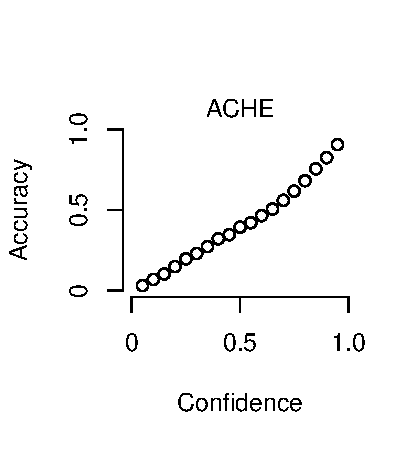
\includegraphics[width=0.19\textwidth]{figures/calibration_plots/ache_calib.pdf}
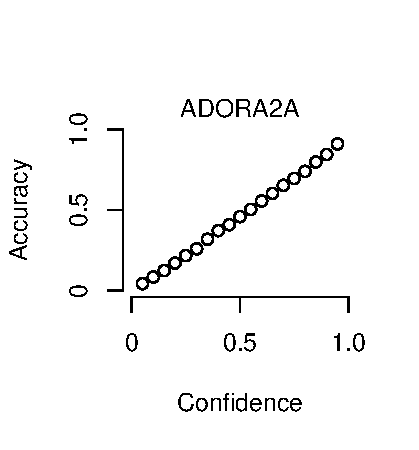
\includegraphics[width=0.19\textwidth]{figures/calibration_plots/adora2a_calib.pdf}
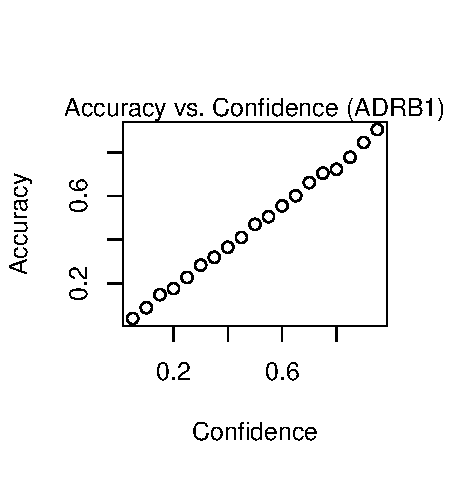
\includegraphics[width=0.19\textwidth]{figures/calibration_plots/adrb1_calib.pdf}
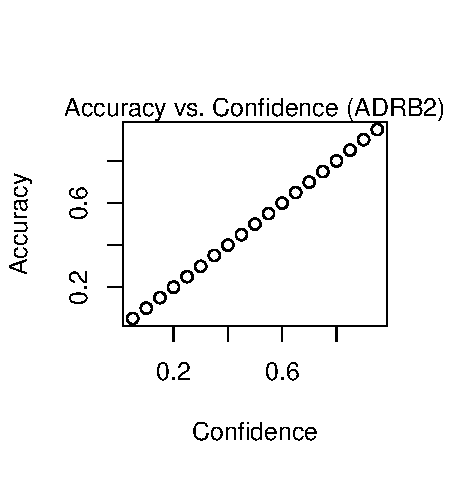
\includegraphics[width=0.19\textwidth]{figures/calibration_plots/adrb2_calib.pdf}
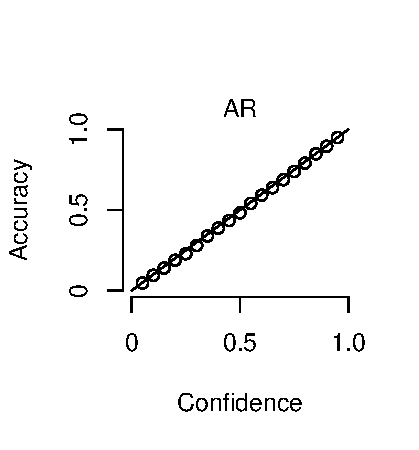
\includegraphics[width=0.19\textwidth]{figures/calibration_plots/ar_calib.pdf}
\vspace*{-15pt} % This is cheating, top margin should be holy, but this table is HUGE!
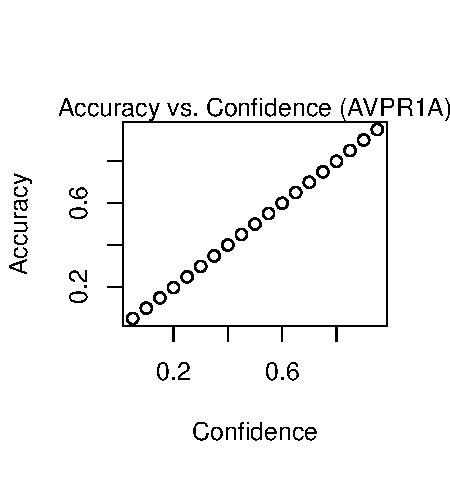
\includegraphics[width=0.19\textwidth]{figures/calibration_plots/avpr1a_calib.pdf}
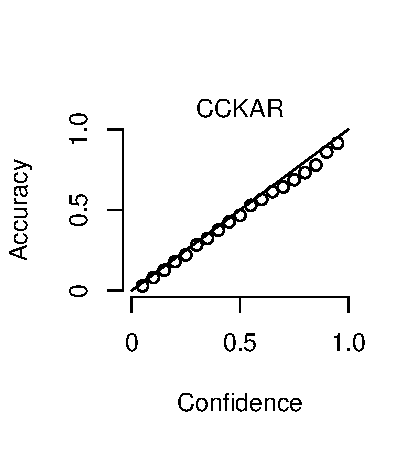
\includegraphics[width=0.19\textwidth]{figures/calibration_plots/cckar_calib.pdf}
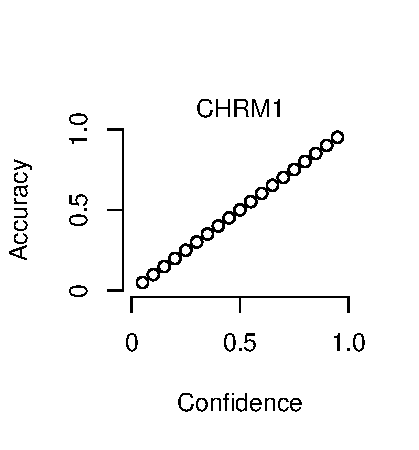
\includegraphics[width=0.19\textwidth]{figures/calibration_plots/chrm1_calib.pdf}
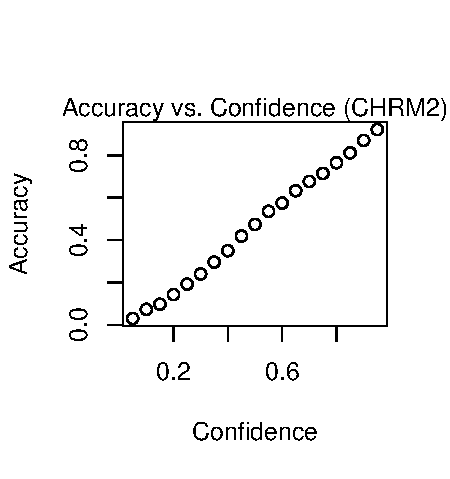
\includegraphics[width=0.19\textwidth]{figures/calibration_plots/chrm2_calib.pdf}
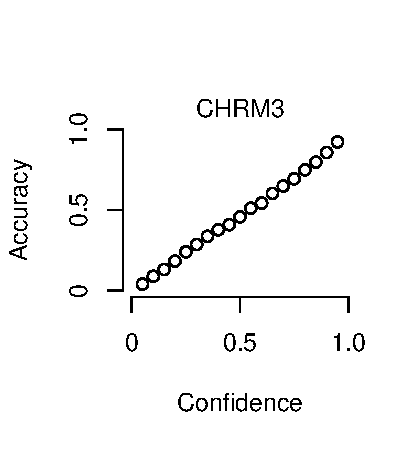
\includegraphics[width=0.19\textwidth]{figures/calibration_plots/chrm3_calib.pdf}
\vspace*{-15pt} % This is cheating, top margin should be holy, but this table is HUGE!
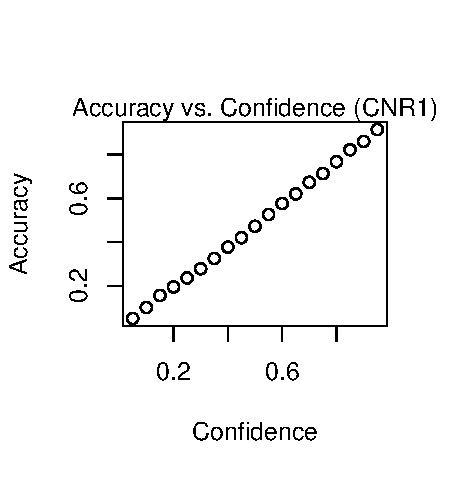
\includegraphics[width=0.19\textwidth]{figures/calibration_plots/cnr1_calib.pdf}
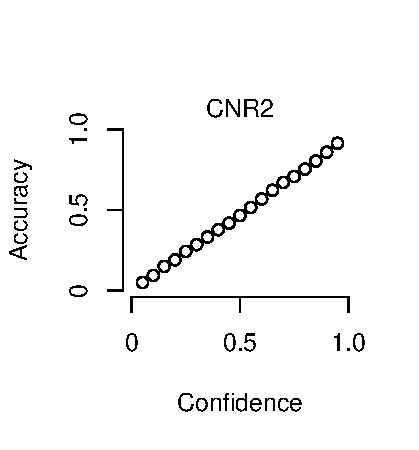
\includegraphics[width=0.19\textwidth]{figures/calibration_plots/cnr2_calib.pdf}
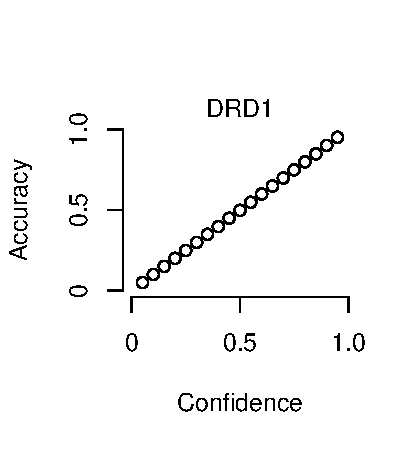
\includegraphics[width=0.19\textwidth]{figures/calibration_plots/drd1_calib.pdf}
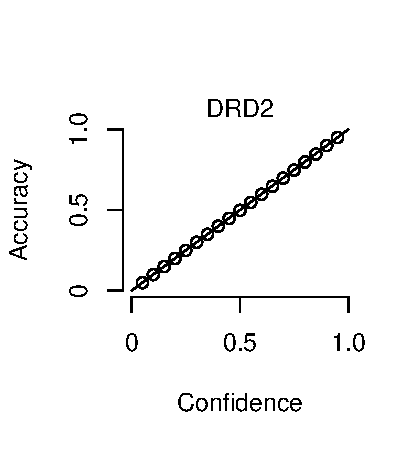
\includegraphics[width=0.19\textwidth]{figures/calibration_plots/drd2_calib.pdf}
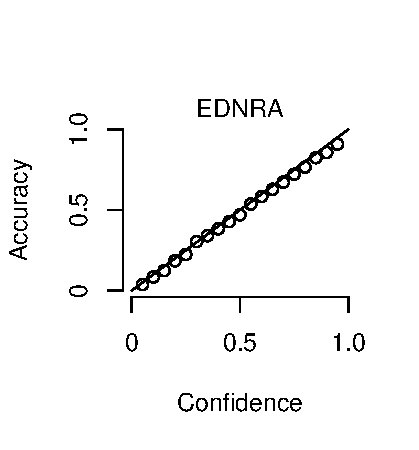
\includegraphics[width=0.19\textwidth]{figures/calibration_plots/ednra_calib.pdf}
\vspace*{-15pt} % This is cheating, top margin should be holy, but this table is HUGE!
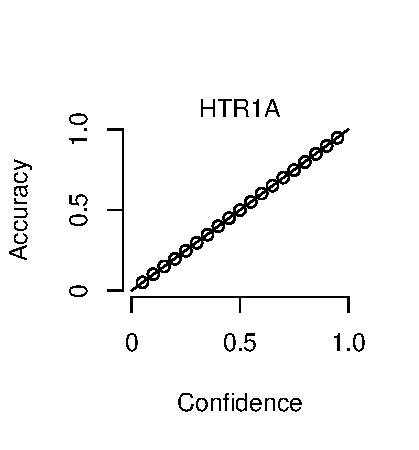
\includegraphics[width=0.19\textwidth]{figures/calibration_plots/htr1a_calib.pdf}
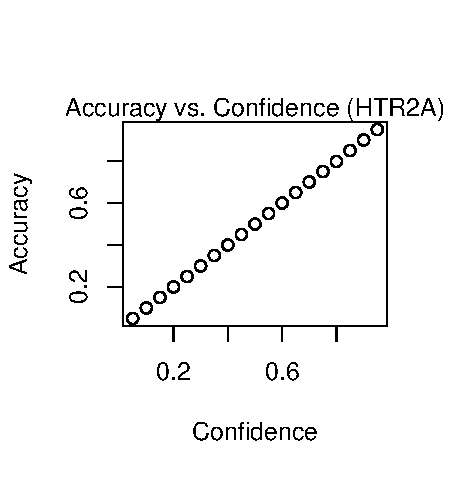
\includegraphics[width=0.19\textwidth]{figures/calibration_plots/htr2a_calib.pdf}
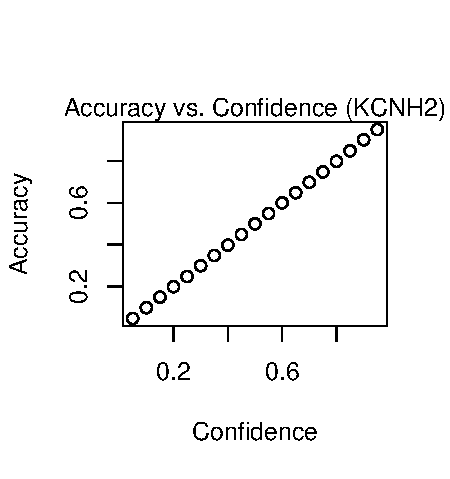
\includegraphics[width=0.19\textwidth]{figures/calibration_plots/kcnh2_calib.pdf}
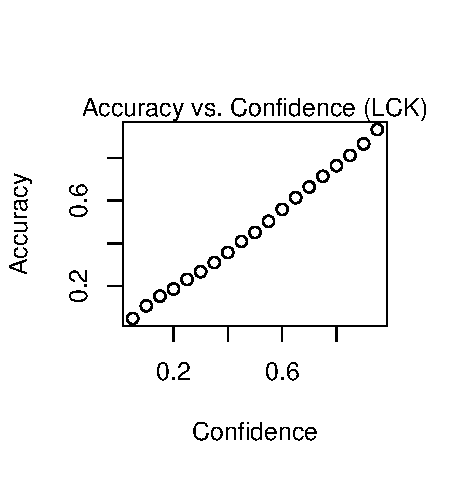
\includegraphics[width=0.19\textwidth]{figures/calibration_plots/lck_calib.pdf}
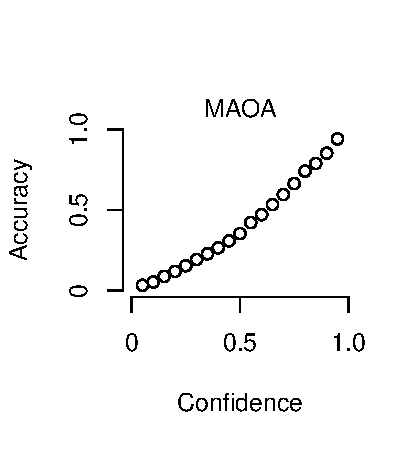
\includegraphics[width=0.19\textwidth]{figures/calibration_plots/maoa_calib.pdf}
\vspace*{-15pt} % This is cheating, top margin should be holy, but this table is HUGE!
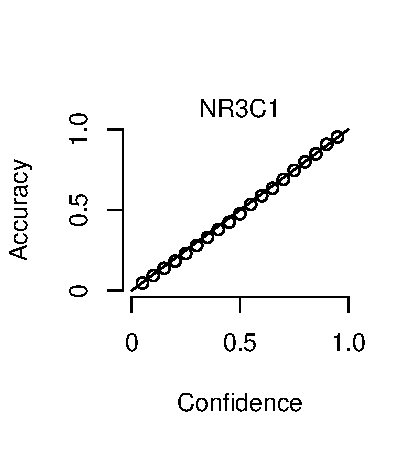
\includegraphics[width=0.19\textwidth]{figures/calibration_plots/nr3c1_calib.pdf}
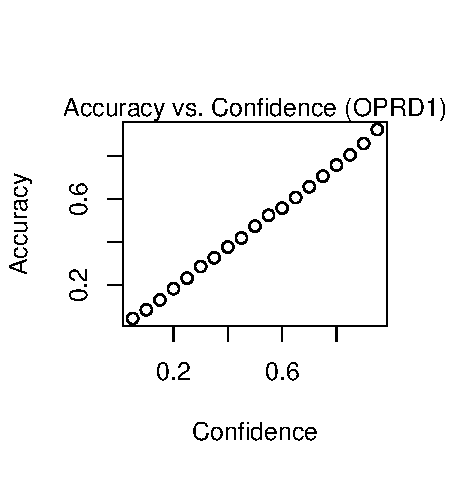
\includegraphics[width=0.19\textwidth]{figures/calibration_plots/oprd1_calib.pdf}
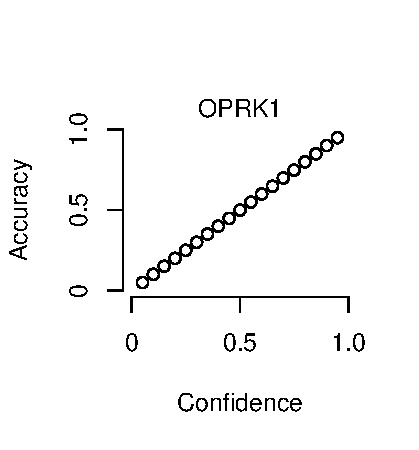
\includegraphics[width=0.19\textwidth]{figures/calibration_plots/oprk1_calib.pdf}
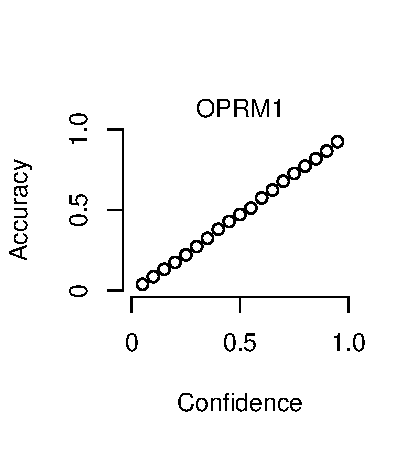
\includegraphics[width=0.19\textwidth]{figures/calibration_plots/oprm1_calib.pdf}
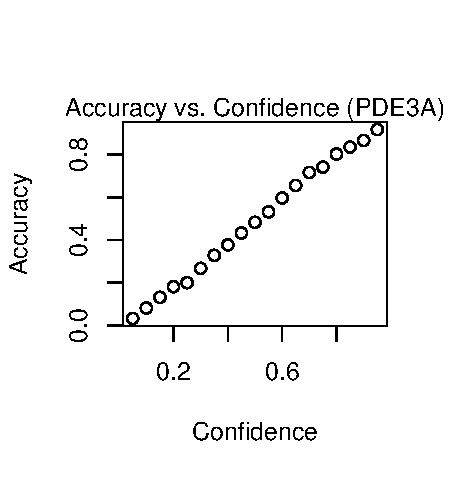
\includegraphics[width=0.19\textwidth]{figures/calibration_plots/pde3a_calib.pdf}
\vspace*{-15pt} % This is cheating, top margin should be holy, but this table is HUGE!
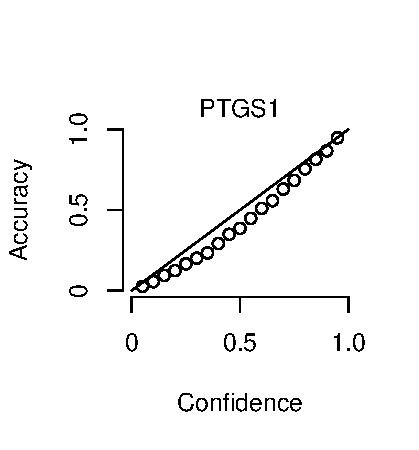
\includegraphics[width=0.19\textwidth]{figures/calibration_plots/ptgs1_calib.pdf}
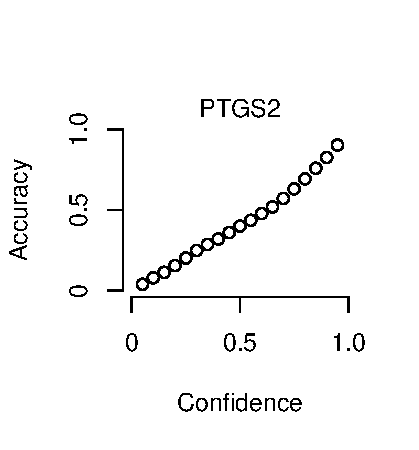
\includegraphics[width=0.19\textwidth]{figures/calibration_plots/ptgs2_calib.pdf}
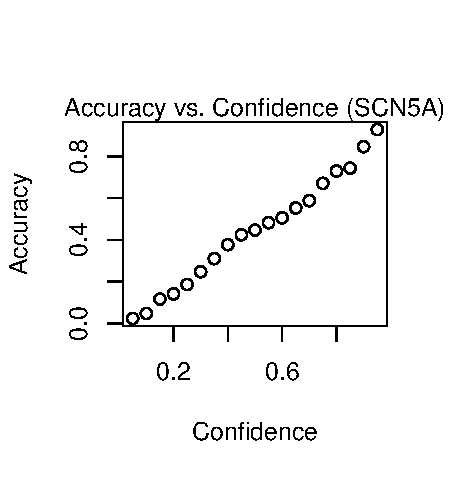
\includegraphics[width=0.19\textwidth]{figures/calibration_plots/scn5a_calib.pdf}
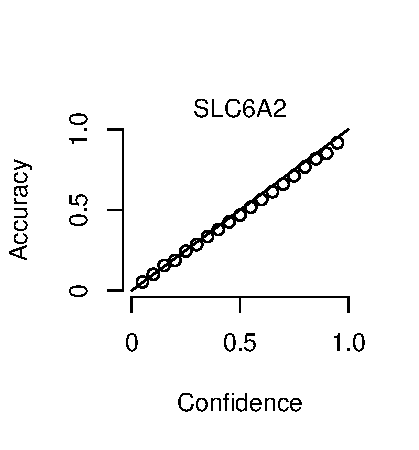
\includegraphics[width=0.19\textwidth]{figures/calibration_plots/slc6a2_calib.pdf}
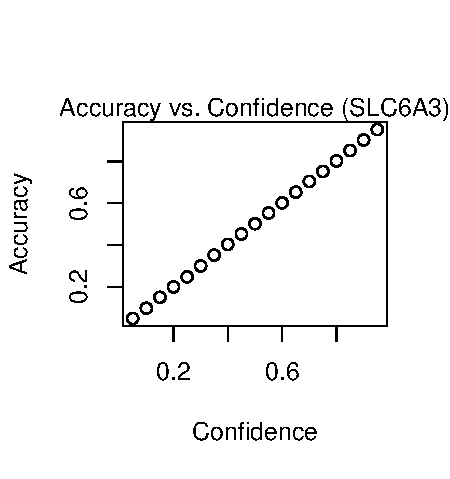
\includegraphics[width=0.19\textwidth]{figures/calibration_plots/slc6a3_calib.pdf}
\vspace*{-15pt} % This is cheating, top margin should be holy, but this table is HUGE!
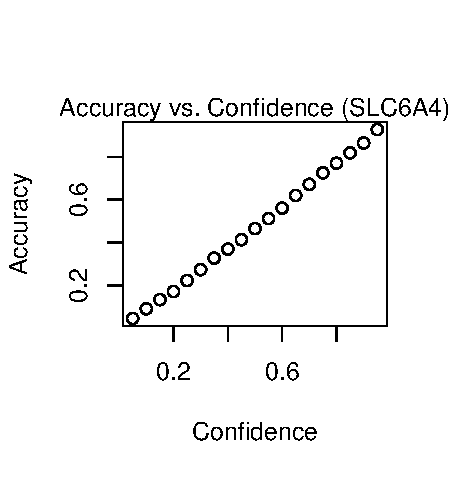
\includegraphics[width=0.19\textwidth]{figures/calibration_plots/slc6a4_calib.pdf}
    \caption{Calibration plots for all targets. The plots show accuracy against
        confidence, for confidence values 0.05 to 0.95 with a step size of 0.05.}
    \label{fig:calplots_all}
\end{figure}

Supplemental 2: Predicted versus observed labels, at confidence level 0.8,
    for all targets \ref{fig:valplots_all_0.8}.

\begin{figure}[h!]

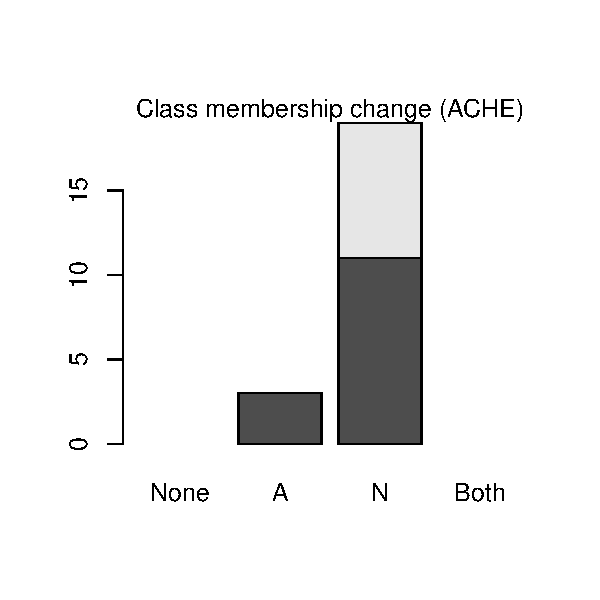
\includegraphics[width=0.15\textwidth]{figures/validation_plots/ache_0p8_valplot.pdf}
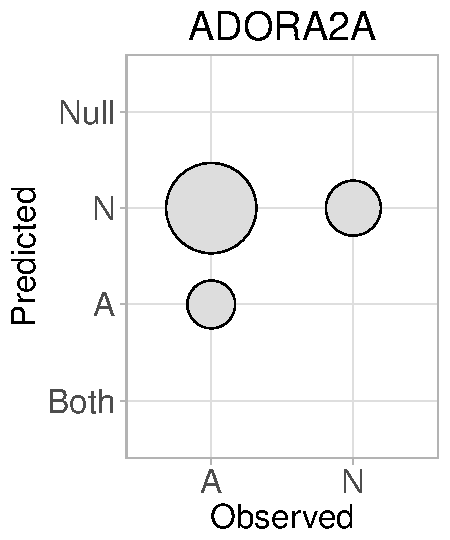
\includegraphics[width=0.15\textwidth]{figures/validation_plots/adora2a_0p8_valplot.pdf}
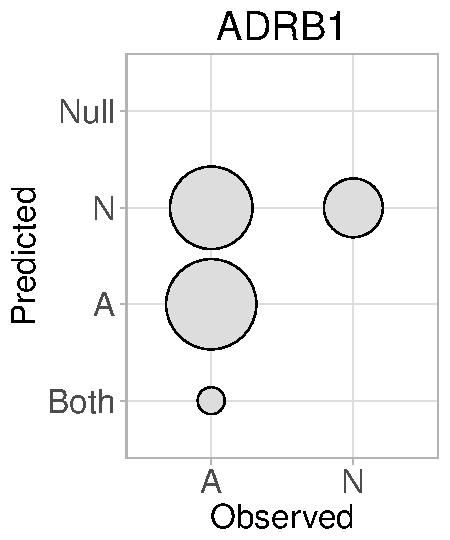
\includegraphics[width=0.15\textwidth]{figures/validation_plots/adrb1_0p8_valplot.pdf}
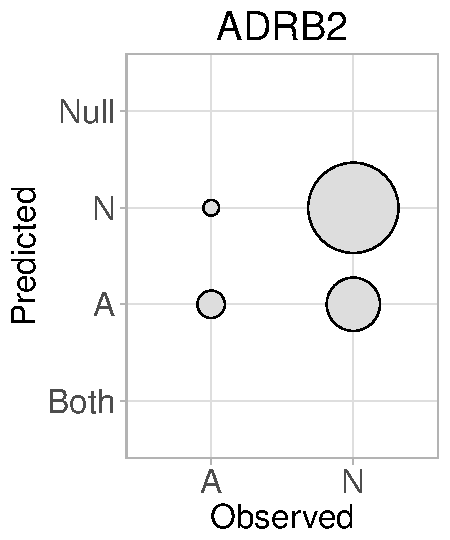
\includegraphics[width=0.15\textwidth]{figures/validation_plots/adrb2_0p8_valplot.pdf}
\includegraphics[width=0.15\textwidth]{figures/validation_plots/ar_0p8_valplot.pdf}
\includegraphics[width=0.15\textwidth]{figures/validation_plots/avpr1a_0p8_valplot.pdf}
\vspace*{10pt} % This is cheating, top margin should be holy, but this table is HUGE!
\includegraphics[width=0.15\textwidth]{figures/validation_plots/cckar_0p8_valplot.pdf}
\includegraphics[width=0.15\textwidth]{figures/validation_plots/chrm1_0p8_valplot.pdf}
\includegraphics[width=0.15\textwidth]{figures/validation_plots/chrm2_0p8_valplot.pdf}
\includegraphics[width=0.15\textwidth]{figures/validation_plots/chrm3_0p8_valplot.pdf}
\includegraphics[width=0.15\textwidth]{figures/validation_plots/cnr1_0p8_valplot.pdf}
\includegraphics[width=0.15\textwidth]{figures/validation_plots/cnr2_0p8_valplot.pdf}
\vspace*{10pt} % This is cheating, top margin should be holy, but this table is HUGE!
\includegraphics[width=0.15\textwidth]{figures/validation_plots/drd1_0p8_valplot.pdf}
\includegraphics[width=0.15\textwidth]{figures/validation_plots/drd2_0p8_valplot.pdf}
\includegraphics[width=0.15\textwidth]{figures/validation_plots/ednra_0p8_valplot.pdf}
\includegraphics[width=0.15\textwidth]{figures/validation_plots/htr1a_0p8_valplot.pdf}
\includegraphics[width=0.15\textwidth]{figures/validation_plots/htr2a_0p8_valplot.pdf}
\includegraphics[width=0.15\textwidth]{figures/validation_plots/kcnh2_0p8_valplot.pdf}
\vspace*{10pt} % This is cheating, top margin should be holy, but this table is HUGE!
\includegraphics[width=0.15\textwidth]{figures/validation_plots/lck_0p8_valplot.pdf}
\includegraphics[width=0.15\textwidth]{figures/validation_plots/maoa_0p8_valplot.pdf}
\includegraphics[width=0.15\textwidth]{figures/validation_plots/nr3c1_0p8_valplot.pdf}
\includegraphics[width=0.15\textwidth]{figures/validation_plots/oprd1_0p8_valplot.pdf}
\includegraphics[width=0.15\textwidth]{figures/validation_plots/oprk1_0p8_valplot.pdf}
\includegraphics[width=0.15\textwidth]{figures/validation_plots/oprm1_0p8_valplot.pdf}
\vspace*{10pt} % This is cheating, top margin should be holy, but this table is HUGE!
\includegraphics[width=0.15\textwidth]{figures/validation_plots/pde3a_0p8_valplot.pdf}
\includegraphics[width=0.15\textwidth]{figures/validation_plots/ptgs1_0p8_valplot.pdf}
\includegraphics[width=0.15\textwidth]{figures/validation_plots/ptgs2_0p8_valplot.pdf}
\includegraphics[width=0.15\textwidth]{figures/validation_plots/scn5a_0p8_valplot.pdf}
\includegraphics[width=0.15\textwidth]{figures/validation_plots/slc6a2_0p8_valplot.pdf}
\includegraphics[width=0.15\textwidth]{figures/validation_plots/slc6a3_0p8_valplot.pdf}
\vspace*{10pt} % This is cheating, top margin should be holy, but this table is HUGE!
\includegraphics[width=0.15\textwidth]{figures/validation_plots/slc6a4_0p8_valplot.pdf}

    \caption{Predicted versus observed labels, at confidence level 0.8,
    for all targets, and all compounds in the prediction dataset.
    The X-axis represents predicted labels, while the Y-axis represents observed values,
    obtained from ExcapeDB. The area of circles is plotted proportional to the number of
    compounds per predicted/observed combination. Note that the scale is different between
    each plot, because of differing total number of compounds per target.
    }
    \label{fig:valplots_all_0.8}
\end{figure}

Supplemental 3: Predicted versus observed labels, at confidence level 0.9,
    for all targets \ref{fig:valplots_all_0.9}.

\begin{figure}[h!]

\includegraphics[width=0.15\textwidth]{figures/validation_plots/ache_0p9_valplot.pdf}
\includegraphics[width=0.15\textwidth]{figures/validation_plots/adora2a_0p9_valplot.pdf}
\includegraphics[width=0.15\textwidth]{figures/validation_plots/adrb1_0p9_valplot.pdf}
\includegraphics[width=0.15\textwidth]{figures/validation_plots/adrb2_0p9_valplot.pdf}
\includegraphics[width=0.15\textwidth]{figures/validation_plots/ar_0p9_valplot.pdf}
\includegraphics[width=0.15\textwidth]{figures/validation_plots/avpr1a_0p9_valplot.pdf}
\vspace*{10pt} % This is cheating, top margin should be holy, but this table is HUGE!
\includegraphics[width=0.15\textwidth]{figures/validation_plots/cckar_0p9_valplot.pdf}
\includegraphics[width=0.15\textwidth]{figures/validation_plots/chrm1_0p9_valplot.pdf}
\includegraphics[width=0.15\textwidth]{figures/validation_plots/chrm2_0p9_valplot.pdf}
\includegraphics[width=0.15\textwidth]{figures/validation_plots/chrm3_0p9_valplot.pdf}
\includegraphics[width=0.15\textwidth]{figures/validation_plots/cnr1_0p9_valplot.pdf}
\includegraphics[width=0.15\textwidth]{figures/validation_plots/cnr2_0p9_valplot.pdf}
\vspace*{10pt} % This is cheating, top margin should be holy, but this table is HUGE!
\includegraphics[width=0.15\textwidth]{figures/validation_plots/drd1_0p9_valplot.pdf}
\includegraphics[width=0.15\textwidth]{figures/validation_plots/drd2_0p9_valplot.pdf}
\includegraphics[width=0.15\textwidth]{figures/validation_plots/ednra_0p9_valplot.pdf}
\includegraphics[width=0.15\textwidth]{figures/validation_plots/htr1a_0p9_valplot.pdf}
\includegraphics[width=0.15\textwidth]{figures/validation_plots/htr2a_0p9_valplot.pdf}
\includegraphics[width=0.15\textwidth]{figures/validation_plots/kcnh2_0p9_valplot.pdf}
\vspace*{10pt} % This is cheating, top margin should be holy, but this table is HUGE!
\includegraphics[width=0.15\textwidth]{figures/validation_plots/lck_0p9_valplot.pdf}
\includegraphics[width=0.15\textwidth]{figures/validation_plots/maoa_0p9_valplot.pdf}
\includegraphics[width=0.15\textwidth]{figures/validation_plots/nr3c1_0p9_valplot.pdf}
\includegraphics[width=0.15\textwidth]{figures/validation_plots/oprd1_0p9_valplot.pdf}
\includegraphics[width=0.15\textwidth]{figures/validation_plots/oprk1_0p9_valplot.pdf}
\includegraphics[width=0.15\textwidth]{figures/validation_plots/oprm1_0p9_valplot.pdf}
\vspace*{10pt} % This is cheating, top margin should be holy, but this table is HUGE!
\includegraphics[width=0.15\textwidth]{figures/validation_plots/pde3a_0p9_valplot.pdf}
\includegraphics[width=0.15\textwidth]{figures/validation_plots/ptgs1_0p9_valplot.pdf}
\includegraphics[width=0.15\textwidth]{figures/validation_plots/ptgs2_0p9_valplot.pdf}
\includegraphics[width=0.15\textwidth]{figures/validation_plots/scn5a_0p9_valplot.pdf}
\includegraphics[width=0.15\textwidth]{figures/validation_plots/slc6a2_0p9_valplot.pdf}
\includegraphics[width=0.15\textwidth]{figures/validation_plots/slc6a3_0p9_valplot.pdf}
\vspace*{10pt} % This is cheating, top margin should be holy, but this table is HUGE!
\includegraphics[width=0.15\textwidth]{figures/validation_plots/slc6a4_0p9_valplot.pdf}

    \caption{Predicted versus observed labels, at confidence level 0.9,
    for all targets, and all compounds in the prediction dataset.
    The X-axis represents predicted labels, while the Y-axis represents observed values,
    obtained from ExcapeDB. The area of circles is plotted proportional to the number of
    compounds per predicted/observed combination. Note that the scale is different between
    each plot, because of differing total number of compounds per target.
    }
    \label{fig:valplots_all_0.9}
\end{figure}

Supplemental 4: Detailed workflow graphs.

Detailed workflow graph for the fillup-vs-not experiment can be seen in figure
\ref{fig:workflow_detailed_fillup_vs_not}.

Detailed workflow graph for the workflow where drugbank compounds were removed,
can be seen in figure \ref{fig:workflow_detailed_wo_drugbank}.

\begin{figure}[h!]
\includegraphics[width=\textwidth]{figures/workflow_graph_fillup_vs_not.pdf}
    \caption{Detailed workflow graph for the fillup-vs-not experiment.}
    \label{fig:workflow_detailed_fillup_vs_not}
\end{figure}

\begin{figure}[h!]
\includegraphics[width=\textwidth]{figures/workflow_graph_wo_drugbank.pdf}
    \caption{Detailed workflow graph for the workflow where drugbank compounds
    were removed. Note the additional components in the top of the figure, for
    preparing and extracting data from the drugbank dataset.}
    \label{fig:workflow_detailed_wo_drugbank}
\end{figure}

\end{document}


